\documentclass[
        a4paper,     % Format A4
        12pt,
        times,
        %titlepage,   % mit Titelseite
        %parskip      % mit Durchschuss
                     % (= Abstand zwischen Absätzen, statt Einrückung)
        ]{article} % KOMA-Script Grundklasse     texdoc scrguide
\usepackage[ngerman,USenglish]{babel}
\usepackage[T1]{fontenc}          % Schriftkodierung mit Umlauten
\usepackage{textcomp,amsmath}     % Mathezeichen etc.
\usepackage{graphicx}             % Graphiken einbinden
\usepackage[utf8]{inputenc}				% direkte Eingabe von Umlauten & Co. (Vorsicht: Encoding im Editor muss auch UTF-8 sein!)
\usepackage{url}
\usepackage{datetime}							% \formatdate
\usepackage{subfig}								% \subfloat
\usepackage{ragged2e}							% \justify

\usepackage[automark]{scrlayer-scrpage} % Page numbers on the right side
\clearpairofpagestyles
\ofoot[\pagemark]{\pagemark}

\usepackage{natbib}

\usepackage[hang]{footmisc} % Consistent footnote indentation for multiline footnotes
\setlength\footnotemargin{10pt}
\usepackage{hyperref}				% Load this after footmisc to prevent footnote warnings

%\pdfsuppresswarningpagegroup=1	% Mutes the warning: "PDF inclusion: multiple PDFs with page group"

\renewenvironment{abstract}[1]
% https://tex.stackexchange.com/questions/151583/how-to-adjust-the-width-of-abstract
 {\small
  \begin{center}
  \bfseries #1\vspace{-.6em}\vspace{0pt}
  \end{center}
  \list{}{
    \setlength{\leftmargin}{.6cm}%
    \setlength{\rightmargin}{\leftmargin}%
  }%
  \item\relax}
 {\endlist}

\newcommand{\sign}[1]{
	%https://tex.stackexchange.com/questions/183698/signature-line-with-dots-and-name-below      
  \begin{tabular}[t]{@{}l@{}}
  \makebox[2.5in]{\dotfill}\\
  \strut#1\strut
  \end{tabular}
}


\UseRawInputEncoding

%\ifsetCustomMargin
%  \RequirePackage[left=37mm,right=30mm,top=35mm,bottom=30mm]{geometry}
%  \setFancyHdr % To apply fancy header after geometry package is loaded
%\fi

% Ragged bottom avoids extra whitespaces between paragraphs
\raggedbottom

\RequirePackage[labelsep=space,tableposition=top]{caption}
\renewcommand{\figurename}{Fig.} %to support older versions of captions.sty

%\usepackage{breakurl}
\usepackage{url}

\usepackage{graphicx}
\usepackage[table,xcdraw]{xcolor}

\usepackage{float}
\restylefloat{table}

\usepackage{makecell}

% Subcaption package is also available in the sty folder you can use that by
% uncommenting the following line
% This is for people stuck with older versions of texlive
%\usepackage{sty/caption/subcaption}
%\usepackage{subcaption}

\usepackage{booktabs} % For professional looking tables
\usepackage{multirow}

%\usepackage{multicol}
%\usepackage{longtable}
%\usepackage{tabularx}
\usepackage{longtable}
\usepackage{siunitx} % use this package module for SI units

\usepackage{natbib,har2nat}
\renewcommand{\bibname}{References}

\setcounter{secnumdepth}{2}
\setcounter{tocdepth}{2}

\usepackage{dcolumn}
\usepackage{multirow}
\usepackage{booktabs}
%\usepackage{epstopdf}
%\usepackage[thinc]{esdiff}
\usepackage{physics}
\usepackage{lmodern}
\usepackage{amsmath}
\usepackage{xcolor}
\usepackage{hyperref}
\usepackage{bm}
\usepackage{listings}
\usepackage{mathptmx}
\usepackage{bibentry}
\usepackage{amsmath,amssymb}
\usepackage{titling}
\usepackage{pythonhighlight}
\usepackage{listings}
%\usepackage{caption}
%\DeclareCaptionType{code}[Code Listing][List of Code Listings] 



%\titlehead{
%\includegraphics{Graphics/test_image.jpg}
%} \subject{Bachelor Thesis}

%\title{The equity risk premium puzzle}
%\author{Gerome Wolf}
%\date{\today}

%\logo{UCL_Banner}
%\title{The equity risk premium puzzle
%\\ \bigskip 
%\large{A cross-country study of asset returns, growth and disaster risk}}
%\author{Gerome Wolf\\ \small{\href{mailto:wolfgerome@gmail.com}{\nolinkurl{wolfgerome@gmail.com}}}}
%\date{\today}
%\publishers{
%Department of Economics\\
%~\\
%\textbf{Supervisors}\\
%Wei Cui}
%Toni Grütze\\
%Michael Loster}



\begin{document}
%\begin{titlingpage}
%\begin{center}
%\begin{lrbox}
%  {
\includegraphics[width = \textwidth]{UCL_Banner} \par}
%\end{lrbox}
%
\includegraphics[width = \textwidth]{UCL_Banner}\\ %Put the logo you want here
%\begin{large}
%University College London \\ %The name your university
%Department of Economics\\
%\end{large}
%\vspace{4cm} %You can control the vertical distance
%\begin{large} 
%\end{large}
%\textbf{\thetitle}\\
%\theauthor\\
%\vspace{7cm} %Put the distance you need.
%\thedate
%\end{center}
%\end{titlingpage}
%
%\title{My title}
%
%\author{My name}
%
%\titlepic{
\includegraphics[width=\textwidth]{UCL_Banner}}
%
%\date{\today} 
%
%\maketitle
\makeatletter
\newcommand\HUGE{\@setfontsize\Huge{28}{30}} 
\makeatother

\begin{titlepage}
   \begin{center}

		
\includegraphics[width=1\textwidth]{UCL_Banner}   
   
       \vspace*{1cm}
		
		\HUGE
		\textbf{The equity risk premium puzzle}

       \vspace{0.2cm}
       \Large
       \textbf{A cross-country study of asset returns, growth and disaster risk}
            
       \vspace{1cm}

       \textit{Candidate:}\\
       \vspace{0.5em}  
       Gerome Wolf
       
		\vspace{0.5cm}
		
		\textit{Dissertation supervisor:}\\
		\vspace{0.5em}  
       Wei Cui
		
       %\vfill
       \vspace{1cm}
       
       \large
       Department of Economics\\
       \vspace{0.5em}  
       University College London\\
       
       \vfill
       
        \vspace{1cm}   
       Dissertation submitted in part-fulfilment of the\\
       \vspace{0.5em}  
       \textit{MSc in Economics}
            
       \vspace{1cm}
            
       \today
       
       \vspace{1cm}
       
       Word count: 9996
            
   \end{center}
\end{titlepage}

\newpage
%\nobibliography*
\begin{abstract}{Abstract}
The equity risk premium puzzle - even its very existence - is arguably one of the most fascinating as well as persistent phenomenons in the field of macro finance that has been attempted to rationalise since the famous seminal paper by \citet{Mehra1985}.\\
Following the disaster risk approach initially proposed by \citet{Rietz1988} and further developed by \citet{Barro2006} I conduct a comprehensive study of asset returns, macroeconomic aggregates and moments related to disastrous events covering almost 150 years of financial markets and economic history across 16 developed countries.\\
Whereas previous studies of disaster risk focused on the reconciliation of economic theory and empirical data using a) aggregate output and b) rationalising the puzzle at a global level my contribution is twofold:

Firstly, I extend the analysis to private consumption expenditure data, a more accurate measure for consumption-based asset pricing for a now-available greater time horizon and secondly I allow for cross-country heterogeneity in characteristics with respect to disaster propensity/experience.

The major finding of my dissertation is that accounting for the effect of disasters on consumption risk (and output risk) does indeed rationalise the puzzle and country-specific preference parameter estimates are presented along with plausible model predictions for the rates of return on equity and risk-free, short-term government bills which appears to attenuate the equity premium puzzle if it also addresses the risk-free rate puzzle \citep{Weil1989} jointly.
\end{abstract}


\newpage
%{\small\tableofcontents}
\tableofcontents
\addtocontents{toc}{\setcounter{tocdepth}{2}}
\newpage
\listoffigures
\listoftables
\newpage
%\addcontentsline{toc}{section}{Introduction}
\section{Introduction} \label{introduction}

The equity risk premium (ERP) puzzle has been arguably one of the most fascinating and persistent topics in modern macroeconomics and finance since its `discovery' by \citet{Mehra1985}, indicating its high relevance to investors, firms, policy makers and the profession of economics alike.

In a binary world (disaster vs. normal), disaster risk \cite{Rietz1988} comprises the decisive `factor' that determines the compensation for being exposed to consumption risk (over being insured against it as governments rarely default on their debt obligations from providing public liquidity) originating from disastrous events only \cite{Nakamura2013}. %Clearly, countries differ in their experienced histories of disaster states and hence capacities to relate to financial markets. 
I identify heterogeneity across 16 developed economies spanning almost 150 years of annual observations with respect to disaster risk, returns and macroeconomic growth rates and fully calibrate a consumption-based asset pricing model incorporating Epstein-Zin-Weil preferences based on the random walk with drift model by \citet{Barro2006} at the country level. 

The underlying idea is that countries with relatively higher probability of entering a disastrous state as well as higher contraction size should compensate investors more than less disaster-risky countries. I identify disaster periods according to an NBER-style peak-to-trough procedure which allows disasters to unfold over multiple years rather than occurring instantaneously which has been addressed by \citet{Julliard2012}.

Uncovering heterogeneity in preferences implied by within-country risk-sharing capacity may shed light on structural differences with respect to risk-carrying and tests the model's ability to rationalize the `puzzle' at smaller units. I show that accounting for time-invariant disaster risk does indeed attenuate the `puzzle' in the sense of a) reducing the implied coefficients of relative risk aversion significantly compared to the benchmark specification proposed in \citet{Mehra1985} and further developed in \citet{Mehra2003} and b) yielding robust and plausible model predictions. 

Moreover, the relative order of implied coefficients of relative risk aversion is being preserved compared to the benchmark specification. 
As \citet{Barro2006} and \citet{Cochrane2017} correctly point out, incorporating stochastic variations in the disaster probability $p_{t}$ would help to explain business-cycle related return predictability and stock price volatility. In my quantitative analysis I treat disaster risk moments as constants (implying that normal and jump shocks are i.i.d. across time and countries and permanent) to provide a baseline estimation at the country level. 

However, \citet{Nakamura2013} incorporate a) consumption data, b) multi-period disasters, c) disaster probability estimation using Bayesian Markov-Chain Monte-Carlo methods and d), most importantly, allow for partial recoveries after crises and therefore address a shortcoming of the \cite{Barro2006} random-walk model which tends to overstate the riskiness of consumption that translates into substantially larger welfare costs of economic fluctuations \cite{Barro2009} as well as higher ERP, at the global level. Accounting for c) and d) is beyond the scope of this paper but \citet{Nakamura2013} argue that it allows for predictability of consumption growth during disasters (which stresses the role of the IES) and reduces the implied coefficient of relative risk aversion to 6.4 and an intertemporal elasticity of substitution of 2.

In consumption-based asset pricing theory where (risk-averse) agents hold assets for the sole purpose of providing future consumption \cite{Abel1991}, optimally when the marginal utility of accessing it is the highest and thus allows for consumption smoothing, combined with general insights from portfolio theory \cite{Markowitz1952} there must be a relationship between characteristics of asset returns and consumption, precisely captured by the so-called stochastic discount factor (volatility) and approximately captured by aggregate consumption (volatility). This is precisely where the puzzle arises: basic consumption-based asset pricing theory cannot be reconciled with the empirical observations, assuming `plausible' values for preferences with respect to risk aversion. The historically observed ERP, originally and most frequently assessed for the US economy \cite{Mehra1985, Cecchetti1993} is too high compared to the model's predicted level for `plausible' values for the coefficient of relative risk aversion (CRRA) and the historically low variability in aggregate consumption expenditures (for a modified version of the original model see \citet{Mehra2003}). 
%Also, the puzzle lies therein that even knowing that investors are more than sufficiently (given the overall degree of risk in the asset markets to consumption) compensated for holding risky assets, overall demand does not show that action is taken accordingly. Quite on the contrary, increased demand for risk-free assets during the past three decades has been partially driving returns globally close to zero \cite{Jorda2017}.

Apart from theoretical and rather technical aspects ``the real risk-adjusted returns on different asset classes reflect equilibrium resource allocations given society’s investment and consumption choices over time'' \cite{Jorda2017} and involves debates about inequality \cite{Piketty2015}, secular stagnation \cite{Summers2014} and the real rate of interest \cite{Holston2017}. Subtly, the ERP is cause and consequence in its own right. Specifically, it represents the excess return of holding a risky asset over the risk-free rate, or, in other words, the opportunity cost of not participating in a risky lottery, investors demand or expect to receive \textit{in turn} affecting asset prices \textit{in turn} affecting returns and the ERP. In the long run, therefore, the level of the ERP should approach its equilibrium value solely determined by preferences and consumption-related volatility.

The paper will proceed as follows: the remainder of this section will lay the theoretical foundation for an accurate treatment of the objects of interest where section \ref{Risk premium theory} abstracts from asset markets and describes the behaviour and existence of a risk premium from a microeconomic perspective. Section \ref{Asset pricing theory} presents the benchmark asset pricing equations under expected power utility that initially gave rise to the aforementioned puzzle. Subsection \ref{disaster risk theory} introduces the asset pricing model accounting for economic disasters. Section \ref{Data} presents the key global and cross-sectional moments and dynamics of international financial markets data as well as macroeconomic aggregates along with disaster model specific moments in the cross-section. Section \ref{Results} presents the results from a baseline calibration with special attention paid to the coefficient of relative risk aversion and rates of return. Sensitvity analyses are performed without altering the main results. Section \ref{Conclusion} concludes with a brief discussion of the paper's implications for international risk-sharing, fiscal capacity as well as liquidity constraints.


\subsection{Risk premium theory} \label{Risk premium theory}
Many modern applications and past advances in economics rest on the expected utility paradigm, that is assuming an additive, time-separable utility representation. In the light of a static lottery with an uncertain outcome over final wealth/consumption and a risk-averse individual there exists a (positive) risk premium as defined as the difference between the expected value and the preference-specific certainty equivalent. Assuming risk-aversion translates into diminishing marginal utility, a reasonable and general description of human behaviour and satisfies strict concavity of the utility function. The very fact of facing an unknown outcome reduces the received utility already as decreasing departures from the mathematical expected value are marginally weighted higher in terms of (dis-)utility than increasing departures from the expected value. %Lower outcomes are therefore more `painful' than higher outcomes contribute to overall felicity. 
Of course, the individual always has the opportunity to opt out of the lottery \textbf{and} maintain the same level of utility \textit{as-if} she would participate. Faced with this choice problem (participating in the risky lottery vs. not participating) one can determine the amount of an e.g. monetary transfer in order to eliminate all uncertainty that would need to occur such that the individual is exactly indifferent between either action as characterized by the level where expected utility of the lottery and utility of initial wealth less the risk premium are equalized.

Clearly, the higher the degree of risk aversion (or the degree of curvature of the utility function) the higher the price an individual is willing to pay to eliminate uncertainty, i.e. the risk premium would be higher. A common utility specification is of the class of isoelastic functions, that is 
\begin{align*}
    u(c)=
    \begin{cases}
        \frac{c^{1-\gamma}}{1-\gamma},& \text{if } \gamma > 0\\
        ln(c), & \text{if } \gamma = 1\\
        0, & \text{otherwise}
    \end{cases}
\end{align*}
which is the standard CRRA utility with desirable properties from a mathematical point of view. Due to strict concavity ($\gamma > 0$) Jensen's inequality establishes the existence of a positive risk premium and allows for closed form solutions to the representative agent's first order conditions (see section \ref{Asset pricing theory}), directly relating risk aversion to asset and consumption characteristics. Also note that the Arrow-Pratt index of relative risk aversion 
\begin{align*}
    -\frac{u''(c) c}{u'(c)} &= \gamma
\end{align*}
which shows that the function is unique up to an affine transformation and basically says that the representative agent's FOC remains unchanged since marginal utilities move in perfect tandem and is therefore independent of the level of initial wealth.

From a social science perspective, however, some assumptions or restrictions implicitly introduced with this functional form are problematic. For example, it introduces a restriction on the intertemporal elasticity of substitution (IES, denoted by $\psi > 0$) which needs to equal the inverse of the coefficient of relative risk aversion, $\gamma$, as shown below:
\begin{align*}
    \psi &= \pdv{ln(c_{t+1}/c_{t})}{r} = -\pdv{ln(c_{t+1}/c_{t})}{ln(u'(c_{t+1} / u'(c_{t})))} = \frac{1}{\gamma}
\end{align*}
where I have used that
\begin{align*}
    R &= \frac{u'(c_{t})}{\beta u'(c_{t+1})} \quad \text{and} \quad ln(R) = r = -ln\left(\frac{u'(c_{t+1})}{u'(c_{t})}\right) - ln(\beta)
\end{align*}
In other words this ``behaviorally groundless restriction'' \cite{Weil1989} means that a highly risk-averse individual has an implicit preference to strongly smooth consumption over time/states of the world by becoming more irresponsive to intertemporal incentives such as the interest rate as risk aversion increases and constant consumption growth becomes the main motive, i.e.
\begin{align*}
    \pdv{\frac{c_{t+1}}{c_{t}}}{R}{\gamma} < 0
\end{align*}
This shortcoming has been recognized early on by \citet{Kreps1978}, \citet{Epstein1989} and \citet{Weil1989} and a generalised form of expected utility has been proposed on which the model calibrated in this paper builds. 
%In any case the theoretical and empirical ERP might be determined by (and determining) preferences with respect to the curvature of the utility function and can be interpreted as the price of aggregate risk to final wealth/consumption derived from a risky lottery's probability distribution.

That the coefficient of relative risk aversion is assumed to be constant is not natural. For example risk aversion could be specified in absolute terms, i.e. portfolio allocations are made with respect to levels as initial wealth increases rather than weights, or (relative) risk aversion could be assumed to decrease as initial wealth increases. Empirical justification for the working assumption of CRRA has been provided by \citet{Brunnermeier2008} and \citet{Chiappori2011}, though. 
%Also note that `constant' does not mean that the coefficient of relative risk aversion is invariant at all; it simply means that it is constant for any level of initial wealth. 
The coefficient of relative risk aversion can (and does) fluctuate over the business cycle as wealth fluctuates \cite{Brunnermeier2008, Gourio2012}.

\subsection{Asset pricing theory} \label{Asset pricing theory}
As has been already asserted, risk-averse agents dislike extreme levels of consumption contemporaneously and would like to, if they cannot fully eliminate it, minimize this variation at least by reducing risk. They can diversify their future-postponed contingent consumption, also referred to as invested wealth into assets that are independently affected by unfavorable downside events. When faced with the decision between an undiversified portfolio and a diversified one with the same expected return the risk averse agent would prefer the diversified one, since it has a lower variance, conditional that a) the events truly affect the individual components of the portfolio independently (or are mutually-exclusive) and b) the correlation of the individual returns is less than 1. In a well-functioning asset market any investor can achieve diversification individually and full diversification is possible in the sense that only aggregate risk to consumption remains where events aren't independent anymore but affect everyone alike, which matches the meaning of market completeness \cite{Constantinides2003}. Implicitly through diversifying the individual allocated some part of the entire risk associated with one asset to the market (`risk-spreading'), simply by not holding it entirely, where another individual holds part of the asset and is exposed to its risk proportionally to the value held. The preference for diversification is intrinsically equivalent to risk aversion as it aims to strike the optimal balance between risk and return, meaning keeping expected return constant but reducing variance, also referred to as mean-preserving spread, or in economic speech to maximize the net effect of additional expected utility from reallocating one probability unit of loss towards the mean (here: expected, mathematical value) and decreased expected utility from reallocating one probability unit of gains towards the mean \cite{Eeckhoudt2011}. 
%Hence, any risk averse investor would follow this strategy since only then it would hold that the utility of the expected value of a lottery is greater or equal but never smaller than expected utility of this lottery, which is, by definition, the characteristic of risk aversion.

\subsubsection{Power utility} \label{Power utility}
It is sensible to start with the fundamental asset pricing equation (FAPE) which describes an investor's first-order condition under standard, expected power utility:
\begin{align*}
    p_t &= \mathop{\mathbb{E}_{t}} (m_{t+1} x_{t+1}) \quad \text{where} \quad m_{t+1} = \beta \frac{u'(c_{t+1})}{u'(c_{t})} \quad \text{and} \quad x_{t+1} = p_{t+1} + d_{t+1}
\end{align*}
The stochastic discount factor $m_{t+1}$ is generally unobservable but its moments can be approximated by making use of the presumption that consumption is log-normally distributed (i.e. consumption growth is i.i.d.) and the CRRA form, yielding the \citet{Hansen1991} bounds and a closed form solution for the risk-free rate (in continuous time):
\begin{align*}
    r_{t}^{f} &= \rho + \gamma \mathop{\mathbb{E}_{t}}(\Delta ln(c_{t+1})) - \frac{1}{2} \gamma (\gamma + 1) \sigma_{t}^{2} (\Delta ln(c_{t+1}))
\end{align*}
which shows that the risk-free rate is determined by preferences ($\beta = \frac{1}{1+\rho}$ and $\gamma$) as well as precautionary savings due to uncertain consumption growth. To match the historically low level of real interest rates and low variability of consumption growth risk aversion would have to be sufficiently small, $\gamma \in [1,5]$ \cite{Cochrane2005}. Moreover, ignoring the third (precautionary savings) term, the second, linear term which is the product of the coefficient of relative risk aversion and the expected growth rate of consumption is positive, requiring $\rho$ to be small or even negative which is the \textit{risk-free rate puzzle} \cite{Weil1989}.\\
\\
In their original paper \citet{Mehra1985} deploy a variation of \citet{Lucas1978} endowment economy and assume that \textit{the growth rate} of endowment follows a Markov process, not the \textit{level}. The Euler equations for equity and a risk-less one-period bond read
\begin{align*}
    1 &= \mathop{\mathbb{E}_{t}} (m_{t+1} R_{t+1}^{e}) \quad \text{where} \quad R_{t+1}^{e} = \frac{p_{t+1} + d_{t+1}}{p_{t}}\\
    1 &= \mathop{\mathbb{E}_{t}} (m_{t+1} R_{t+1}^{f}) \quad \text{where} \quad R_{t+1}^{f} = \frac{1}{q_t}
\end{align*}
After applying the covariance decomposition on the Euler equations and using that $R_{t+1}^{f} = \frac{1}{\mathop{\mathbb{E}_{t}}m_{t+1}}$ the equity premium equation is given by
\begin{align*}
    \mathop{\mathbb{E}_{t}} (R_{t+1}^{e}) - R_{t+1}^{f} &= -R_{t+1}^{f}\text{Cov}_{t}(m_{t+1}, R_{t+1}^{e}) = -\frac{\text{Cov}_{t}[u'(c_{t+1}), R_{t+1}^{e}]}{\mathop{\mathbb{E}_{t}}(u'(c_{t+1}))} 
\end{align*}
which shows that the expected excess return increases (and the asset's expected price falls) in the covariance between the asset's return and marginal utility of consumption. If this covariance is positive this asset provides \textit{insurance}, making it a very valuable component of intertemporal utility meeting high demand which decreases its rate of return. Conversely, if the asset's returns covary negatively with marginal utility (i.e. it does pay off when consumption is high and marginal utility low) it exacerbates consumption variability and hence works against the consumption smoothing motive inherent from expected utility.

Originally, the authors solve this system of two equations by calibrating a discretized Markov process \cite{Tauchen1986} for consumption growth and allow for values for $\gamma \in [0,10]$ and $\beta \in (0,1)$ . They conclude that ``The largest premium obtainable with the model is 0.35 percent, which is not close to the observed value'' \cite{Mehra1985} which is about 6\%.

In a modified version \cite{Mehra2008} with additional assumptions on the distributions of the growth rates consumption and dividends to be i.i.d. as well as both to be jointly log-normally distributed the (log) asset returns read
\begin{align*}
    ln[\mathop{\mathbb{E}_{t}} (R_{t+1}^{e})] &= \rho + \gamma \mu_{\Delta ln(c_{t+1})} - \frac{1}{2} \gamma^{2} \sigma_{\Delta ln(c_{t+1})}^{2} + \gamma \sigma_{(\Delta ln(c_{t+1}), \Delta ln(d_{t+1}))}\\
    ln(R_{t+1}^{f}) &= \rho + \gamma \mu_{\Delta ln(c_{t+1})} - \frac{1}{2} \gamma^{2} \sigma_{\Delta ln(c_{t+1})}^{2}\\
    ln[\mathop{\mathbb{E}_{t}} (R_{t+1}^{e})] - ln(R_{t+1}^{f}) &= \gamma \sigma_{(\Delta ln(c_{t+1}), \Delta ln(d_{t+1}))}
\end{align*}
where the last equation is the (log) equity risk premium which is the product of the coefficient of relative risk aversion $\gamma$ and the covariance between the growth rate of consumption and growth rate of dividends (or alternatively with the return on equity due to homogeneity of $p_t$ of degree 1 in $d_t$). Using the last generalisation \textbf{and} imposing the equilibrium condition that
\begin{align*}
    \Delta ln(c_{t+1}) &= \Delta ln(d_{t+1})
\end{align*}
i.e. the growth rate of consumption to be perfectly correlated with dividend growth (and hence return on equity) simplifies to
\begin{align*}
    ln[\mathop{\mathbb{E}_{t}} (R_{t+1}^{e})] - ln(R_{t+1}^{f}) &= \gamma \sigma_{\Delta ln(c_{t+1})}^{2}
\end{align*}
which shows that the (log) ERP is equal to the product of the coefficient of relative risk aversion $\gamma$ and the variance of consumption growth. It can be shown that under power utility with $\gamma > 1$ an increase in uncertainty ($\sigma_{\Delta ln(c_{t+1})}^{2}$ and/or disaster risk moments, see section \ref{disaster risk theory}) leads to the implausible prediction of a \textit{higher} price-dividend ratio. This implication originates from the restriction on the IES $\psi = \frac{1}{\gamma}$. To produce plausible predictions the IES needs to be greater than $1$.

\subsubsection{Recursive utility} \label{Recursive utility}
To overcome the aforementioned implicit restriction on the IES a generalised version of expected utility function was initially proposed by \citet{Kreps1978} and further developed by \citet{Epstein1989} and \citet{Weil1989}. 
\begin{align*}
    U_{t}[c_{t}, \mathop{\mathbb{E}_{t}} U_{t+1}] &= \left[(1-\beta) c_{t}^{1-\theta} + \beta(\mathop{\mathbb{E}_{t}} U_{t+1})^{\frac{1-\theta}{1-\gamma}} \right]^{\frac{1-\gamma}{1-\theta}}
\end{align*}
where $\gamma$ is the coefficient of relative risk aversion and $\theta$ captures the inverse of the intertemporal elasticity of substitution, $\psi$, and is independent of $\gamma$. This functional equation essentially allows marginal utilities across states to be dependent. If $\gamma = \theta$ the intertemporal program reduces to the ``standard'' expected utility framework where $\gamma = \frac{1}{\psi}$.
The first-order condition for the representative agent's choices of consumption over time subject to the intertemporal budget constraint 
\begin{align*}
    w_{t+1} = (1+ R_{t+1}^{w})(w_t - c_t)
\end{align*}
where $w_{t+1}$ is the budget of wealth and $(1+R_{t+1}^{w})$ is the gross rate of return on the portfolio of all invested wealth (= the market portfolio) can be shown to be
\begin{align*}
    \beta^{\frac{(1-\gamma)}{(1-\theta)}} \cdot \mathop{\mathbb{E}_{t}} \left\{ \left(\frac{c_{t+1}}{c_{t}}\right)^{-\theta \left(\frac{1-\gamma}{1-\theta}\right)} \cdot R_{w, t+1}^{(\theta-\gamma)/(1-\theta)} \cdot R_{t+1}\right\} = 1
\end{align*}
where $R_{w, t+1}$ is the gross return on overall wealth (in the sense of ownership rights on trees in the Lucas tree model) and $R_{t+1}$ is the gross return on any asset (see \citet{Constantinides2003}).

Proceeding similarly to the expected utility case and assuming that the growth rate of consumption and asset returns are i.i.d. and jointly lognormal gives the following closed form solutions
\begin{align*}
    ln[\mathop{\mathbb{E}_{t}} (R_{t+1}^{e})] &= \zeta \frac{\sigma_{(\Delta ln(d_{t+1}), \Delta ln(c_{t+1}))}}{\psi} + (1-\zeta) \sigma_{(\Delta ln(d_{t+1}), \Delta ln(w_{t+1}))} + ln(R_{t+1}^{f}) - \frac{\sigma_{\Delta ln(d_{t+1})}^{2}}{2}\\
    ln(R_{t+1}^{f}) &= \rho + \frac{1}{\psi} \mathop{\mathbb{E}_{t}}(\Delta c_{t+1}) + \frac{\zeta -1}{2} \sigma_{\Delta ln(w_{t+1})}^{2} - \frac{\zeta}{2\psi^{2}} \sigma_{\Delta ln(c_{t+1})}^{2}
\end{align*}
where $\zeta = \frac{1-\gamma}{1-\frac{1}{\psi}}$ and is equal to 1 iff $\gamma = \frac{1}{\psi}$ and $\Delta ln(w_{t+1})$ is the net return on the portfolio of all invested wealth. Interestingly, this shows that a high degree of risk aversion doesn't require a low average risk-free rate (as compared to the case where $\zeta=1$).
On this note, \citet{Weil1989} asserts that ``with i.i.d. dividend growth, the equity premium, when defined in relative terms, is independent of the IES, and reflects only the properties of the dividend growth process and, of course, the magnitude of the CRRA.''

\subsection{Disaster risk theory} \label{disaster risk theory}
%What is an economic disaster? Obviously, any economic contraction is different with respect to its origin, size, duration, persistence and geography, to name just a few aspects. 
The disaster risk approach rests on the idea that the very possibility of rare but disastrous events such as the Great Depression and wars but also natural catastrophes affects investors' variance of marginal utility and hence prices and returns.

Real output per capita (or real consumption per capita in the closed economy with no investment and government) evolves exogenously as random walk with drift with constant population according to
\begin{align*}
    ln(A_{t+1}) &= ln(A_{t}) + g + u_{t+1} + v_{t+1}
\end{align*}
where $g$ is exogenous productivity growth (average growth rate of the economy during non-disastrous periods), $u_{t+1}$ is i.i.d. normal with mean 0 and variance $\sigma^{2}$, reflecting non-disastrous economic fluctuations due to e.g. productivity shocks. $v_{t+1}$ reflects jump shocks associated with economic disasters and is i.i.d. (also with $u_{t+1}$) which allows for closed-form solutions. As such, ``they represent permanent effects on the level of output, rather than transitory disturbances to the level.'' \cite{Barro2008}

The probability of a disastrous event occurring and hence for $v_{t+1} \neq 0$ is $p$. The disaster size, i.e. the fraction of output's contraction is $b$. The distribution of $v_{t+1}$ is
\begin{align*}
   v_{t+1} =
    \begin{cases}
        0,& \text{with } 1-p\\
        ln(1-b), & \text{with } p
    \end{cases}
\end{align*}
where $p$ is constant, a strong limitation for time-varying risk assessments. Recent research \cite{Tsai2015} addresses this limitation with respect to the \textit{excess volatility puzzle} \cite{Shiller1981}.

The effective expected growth rate of output (or consumption) $g^{*}$ is given by
\begin{align*}
    g^{*} &= g + \frac{1}{2} \sigma^{2} - p \cdot \mathop{\mathbb{E}}(b)
\end{align*}
where $\mathop{\mathbb{E}}(b)$ is the expected value of disastrous contractions.
The representative agent is assumed to maximize utility with Epstein-Zin-Weil preferences and with i.i.d. shocks the first-order conditions reads
\begin{align*}
    c_{t}^{-\gamma} &= \beta^{*} \mathop{\mathbb{E}_{t}}(R_{t} c_{t+1}^{-\gamma})
\end{align*}
where $\beta^{*}$ is the effective subjective discount factor, $\beta^{*} = \frac{1}{1+\rho^{*}}$, $\beta = \frac{1}{1+\rho}$ and the effective time preference rate $\rho^{*}$ is given by
\begin{align*}
    \rho^{*} = \rho - (\gamma - \theta) \cdot \left\{g^{*} - \frac{1}{2} \gamma \sigma^{2} - \left(\frac{p}{\gamma -1}\right) \cdot [\mathop{\mathbb{E}}(1-b)^{1-\gamma}-1-(\gamma-1) \cdot \mathop{\mathbb{E}}(b)]\right\}
\end{align*}
where $\theta = \frac{1}{\psi}$ and $\psi$ is the IES. Intuitively, the (effective) time preference rate can be interpreted as the hypothetical riskless real interest rate that existed if consumption would be constant forever at the level $g^{*}$ and that was known, without growth and variability and the same would hold for disaster risk parameters $p$ and $\mathop{\mathbb{E}}(b)$.

The expected rate of return on equity (unlevered) reads
\begin{align*}
    r^{e} &= \rho^{*} + \gamma g^{*} - \frac{1}{2} \gamma (\gamma-1) \sigma^{2} - p \cdot [\mathop{\mathbb{E}}(1-b)^{1-\gamma}-1-(\gamma-1) \mathop{\mathbb{E}}(b)]
\end{align*}
which increases in the effective time preference rate $\rho^{*}$, the product of the coefficient of relative risk aversion and the effective growth rate of exogenous productivity and decreases in the variability of consumption growth (precautionary savings). The new term accounts for disaster risk which decreases the rate of return on equity as $p$ and $\mathop{\mathbb{E}}(b)$ increase.

The risk-free rate is given by
\begin{align*}
    r^{f} &= \rho^{*} + \gamma g^{*} - \frac{1}{2} \gamma (\gamma+1) \sigma^{2} - p \cdot [\mathop{\mathbb{E}}(1-b)^{-\gamma}-1-\gamma \mathop{\mathbb{E}}(b)]
\end{align*}
The equity premium therefore is
\begin{align*}
    r^{e} - r^{f} &= \gamma \sigma^{2} + p \cdot [\mathop{\mathbb{E}}(1-b)^{-\gamma}-\mathop{\mathbb{E}}(1-b)^{1-\gamma}-\mathop{\mathbb{E}}(b)] = \gamma \sigma^{2} + p \cdot \mathop{\mathbb{E}} \{b \cdot [(1-b)^{-\gamma}-1]\}
\end{align*}
If $\gamma = \theta = \frac{1}{\psi}$ the term inside the curly brackets can be interpreted as the product between the proportionate decline in output and excess marginal utility of consumption in a disaster state over that in a normal state (the term inside the square brackets).

~\\
\section{Data} \label{Data}
The data presented in the following and was used to calibrate the disaster risk model has been taken from \citet{Jorda2017}, who ``painstakingly compiled annual asset return data for 16 advanced countries, over nearly 150 years.'' A current version of the public data set may be found on \textcolor{blue}{\href{http://www.macrohistory.net/data/}{Jordà-Schularick-Taylor Macrohistory Database}} (http://www.macrohistory.net/data/). Moreover, the authors acknowledge the ``largest but often ignored component of household wealth, housing'' and provide total returns data, including housing. Although this component does certainly constitute a capital asset with its own, very specific characteristics affecting the households' consumption-savings decision I will omit it and focus on stock market returns (i.e. out of risky assets) for comparability across countries and the existing literature.

For convenience and familiarisation with the data set I found it useful to develop an own \textcolor{blue}{\href{http://disaster-app-master.herokuapp.com/}{web application}} (http://disaster-app-master.herokuapp.com/) in Python using Dash\footnote{https://plotly.com/dash/, a HTML wrapper framework for building analytical web apps, mainly used in Machine Learning and Data Science drawing from interactive Plotly graphics} for visualisation and exploration. The GitHub repository may be found \textcolor{blue}{\href{https://github.com/gerwolf/macro-disaster}{here}} https://github.com/gerwolf/macro-disaster.

Some corrections had to be applied, in particular for stock market data in Germany during the period of hyperinflation (1914-1924) where outliers were removed and imputed using the real performance index by \citet{Gielen1994} which had a Pearson correlation coefficient of about 0.8 with the Jordà-Schularick-Taylor (JST) measure of real total return on equity between the years 1872 and 1992 excluding the years 1922-1924. Other missing values were imputed using moving averages.

Table \ref{tab:data_coverage} in the appendix describes the availability for each key series, earliest starting in 1870 and in unbalanced cases starting dates were chosen such that they were no different within countries, except for Belgium, Japan and Portugal due to missing consumption data but otherwise complete series.

Altogether, the sample accounts for about 35\% of the world GDP in 2015 (PPP) according to the World Bank database\footnote{Accessed 13/09/2020}. The relative composition inside the sample \footnote{measured in real GDP (PPP) using the Maddison Project dataset}, however, did change considerably between 1900 and 2015. The US increased their contribution from 30\% to 47\% whereas the UK's share decreased by 11\% to 7\% followed by Germany with a reduction of 8\% to 8\%. Japan increased it's proportionate contribution from 5\% to 13\%. At the global level returns and growth data are considered from 1900 to 2015 due to incompleteness of observations and weightings before that date.

\subsection{International financial markets}
Total nominal (gross) returns for asset $i$ in country $j$ at time $t$ were calculated according to
\begin{align*}
    R_{i,j,t} &= \frac{P_{i,j,t} - P_{i,j,t-1}}{P_{i,j,t-1}} + Y_{i,j,t}
\end{align*}
where $P$ is the asset's price and $Y$ is the yield component, e.g. dividends. Total real (net) returns were calculated according to
\begin{align*}
    r_{i,j,t} &= \frac{1+R_{i,j,t}}{1+\pi_{j,t}} - 1
\end{align*}
where $\pi$ is the inflation rate.\\
\\
At the global level (see table \ref{tab:global_returns}), i.e. equally weighted as well as real GDP-value weighted average rates of return, real rates of return on equity outperformed Treasury bills with 6.57\% (7.03\%) equally weighted (real-GDP weighted) compared to -0.39\% (-0.17\%) resulting in an equity risk premium of 6.96\% (7.20\%). Variability was higher for equity than for relatively safe assets by a factor of 3.

{\renewcommand{\arraystretch}{1}
\begin{table}[H]
\begin{center}
\begin{tabular}{rccccccc}
\hline
\hline
 & \multicolumn{3}{c}{All equally weighted} & & \multicolumn{3}{c}{real GDP-weighted} \\
 \cline{2-4} \cline{6-8}
 & Equity & Bills & ERP & &Equity & Bills & ERP \\
\hline
Full sample & & & & & & & \\
\hline

Mean return p.a. & 6.57 & -0.39 & 6.96 & & 7.03 & -0.17 & 7.20\\ 

Std. dev. & 15.43 & 6.28 & 14.66 & & 15.26 & 5.95 & 15.02\\ 

Geometric mean & 5.37 & -0.61 & 5.88 & & 5.86 & -0.36 & 6.07\\ 

Median & 6.68 & 1.07 & 6.97 & & 7.46 & 1.39 & 8.27\\ 

Max & 39.45 & 10.84 & 36.57 & & 48.34 & 11.94 & 47.28\\ 

Min & -46.09 & -28.83 & -46.42 & & -41.38 & -21.44 & -41.20\\ 

Kurtosis & 3.87 & 7.95 & -4.08 & & 3.61 & 6.64 & 3.82\\ 

\hline 
Post-1984 & & & & & & & \\
\hline 

Mean return p.a. & 10.89 & 2.22 & 8.67 & & 9.31 & 1.93 & 7.37\\ 

Std. dev. & 20.39 & 2.34 & 20.27 & & 16.86 & 2.16 & 16.58\\ 

Geometric mean & 8.77 & 2.20 & 6.54 & & 7.84 & 1.91 & 5.94\\ 

Median & 12.02 & 2.15 & 12.14 & & 13.26 & 2.37 & 13.00\\ 

Max & 39.45 & 5.83 & 35.28 & & 33.81 & 5.11 & 32.52\\ 

Min & -46.09 & -1.23 & -46.42 & & -41.38 & -1.83 & -41.20\\ 

Kurtosis & 3.65 & 1.74 & 3.38 & & 4.44 & 1.76 & 4.17\\ 
\hline
\hline
\end{tabular} 
\end{center}
\caption{Global real returns (1900-2015)}
\label{tab:global_returns}
\end{table}

For the post-1984 period subset returns across both asset classes were higher compared to the full sample
%with an unweighted (real-GDP weighted), annual mean return of 10.89\% (9.31\%) for equity and 2.22\% (1.93\%) for Treasury bills. 
Volatility was higher in this period for equity but smaller for T-bills. %Note that the biggest stock market turmoils out of the entire sample occured in the post-1984 period whereas Treasury bills remained stable during that period. Overall, the ERP was 8.67\% in the unweighted sample and 7.37\% in the real-GDP weighted sample.


\begin{figure}[H]
	\begin{tabular}{cc}
	\subfloat[Equity]{
		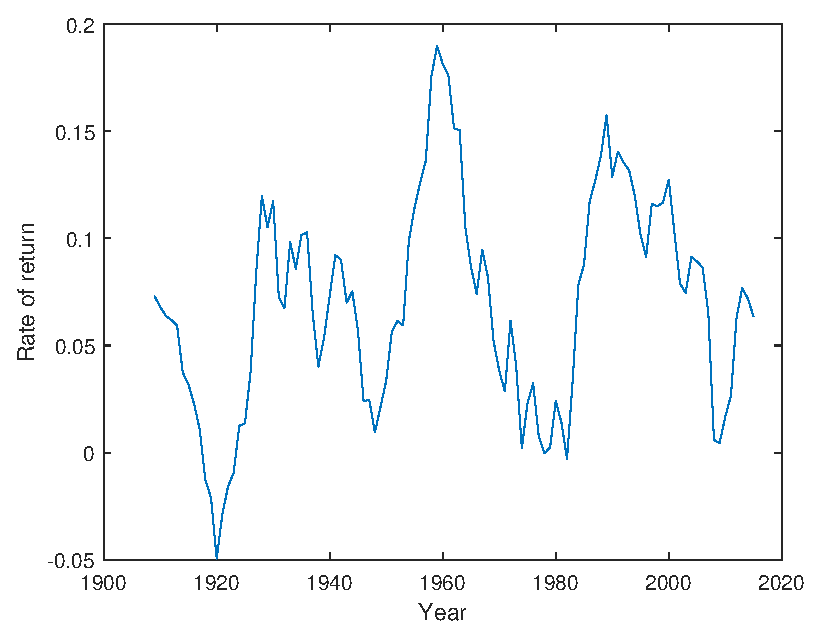
\includegraphics[keepaspectratio = true, width = 0.45\textwidth]{Matlab Graphics/Figure_2_equity}
	} &
	\subfloat[Treasury bills]{
		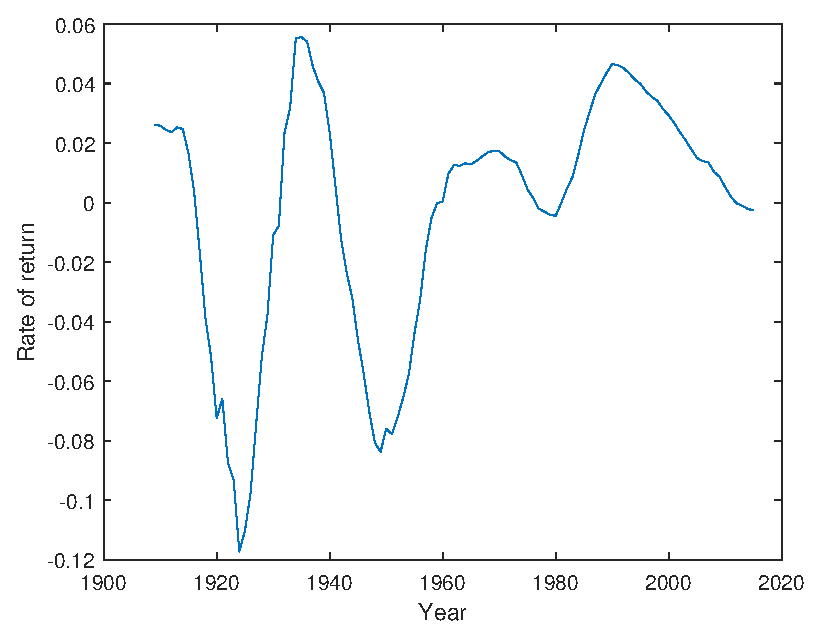
\includegraphics[width = 0.45\textwidth]{Matlab Graphics/Figure_2_bills}
	}\\
	\end{tabular}
	\caption{Decadal, real-GDP weighted moving averages of asset returns}
	\label{fig:decadal_MA_asset_returns}
\end{figure}

Figure \ref{fig:decadal_MA_asset_returns} indicates that returns on equity and T-bills show some cyclical behaviour with equity being more volatile than risk-free rates.\\
\\
At the country-level (see table \ref{tab:real_returns_countries} in the appendix) there is some degree of variation in asset returns; returns on equity range from values as low as 3.02\% (France) to 8.90\% (Finland). Treasury bills returned, on average, -2.57\% (Germany) to 2.99\% (Denmark). Interestingly, German investors lost on average 2.57\% of their initial wealth when holding safe assets \footnote{\citet{Probst2019} estimates the average short-term real interest rate for Germany (1871-2013) even lower at -3.5\%.}. German \textit{Bunds} are recognized as one of the assets with the lowest probability of default, hence making it a valuable asset as it provides (almost) perfect insurance, driving up its price and lowering its return. In total, for seven countries the measured average real risk-free rate was negative.% Similarly to global rates, asset returns were higher during the post-1984 period than in the entire sample period with higher associated volatility, though. 
\newpage
The resulting premiums are documented in table \ref{tab:erp_countries} below:

{\renewcommand{\arraystretch}{1}
\begin{table}[H]
\begin{center}
\begin{tabular}{rccccc}
\hline
\hline
Country & \multicolumn{2}{c}{Full sample (1870-2015)} & & \multicolumn{2}{c}{post-1984} \\
\cline{2-3} \cline{5-6}
& Mean & Std & & Mean & Std\\
\hline
Australia & 6.59 & 15.86 & & 5.13 & 18.76\\
Belgium & 5.91 & 22.89 & & 9.68 & 24.85\\
Denmark & 4.90 & 18.01 & & 8.15 & 22.72\\
Finland & 10.34 & 30.90 & & 12.90 & 42.40\\
France & 4.34 & 21.37 & & 8.02 & 24.45\\
Germany & 10.47 & 36.62 & & 8.50 & 24.96\\
Italy & 6.50 & 30.81 & & 7.09 & 29.80\\
Japan & 9.24 & 27.00 & & 4.20 & 22.56\\
Netherlands & 6.51 & 23.08 & & 8.66 & 22.80\\
Norway & 5.00 & 20.36 & & 10.36 & 29.24\\
Portugal & 4.14 & 27.45 & & 9.44 & 39.37\\
Spain & 6.37 & 21.30 & & 11.84 & 28.31\\
Sweden & 6.45 & 20.00 & & 11.75 & 28.10\\
Switzerland & 5.76 & 18.73 & & 9.39 & 22.51\\
United Kingdom & 5.94 & 19.24 & & 5.75 & 15.45\\
United States & 6.28 & 18.36 & & 7.92 & 16.44\\
\hline
\hline
\end{tabular} 
\end{center}
\caption{Equity risk premium (country-level), \%}
\label{tab:erp_countries}
\end{table}

%The highest risk premium was 10.47\% for Germany, the lowest was 4.14\% for Portugal in the full sample. The global, unweighted ERP was about 6.55\% in the full sample and 8.67\% for the post-1984 period. 
%Variability in the market price of risk did also increase in the post-1984 period, indicating more frequently fluctuating consumption according to the theoretical models described in section \ref{introduction}.
Measuring the intra-sample consistency (by the standardized coefficient of variation across countries) in risk-free rates shows an interesting picture how stable they really were in the past:

\begin{figure}[H]
	\begin{tabular}{cc}
	\subfloat[1900-1983]{
		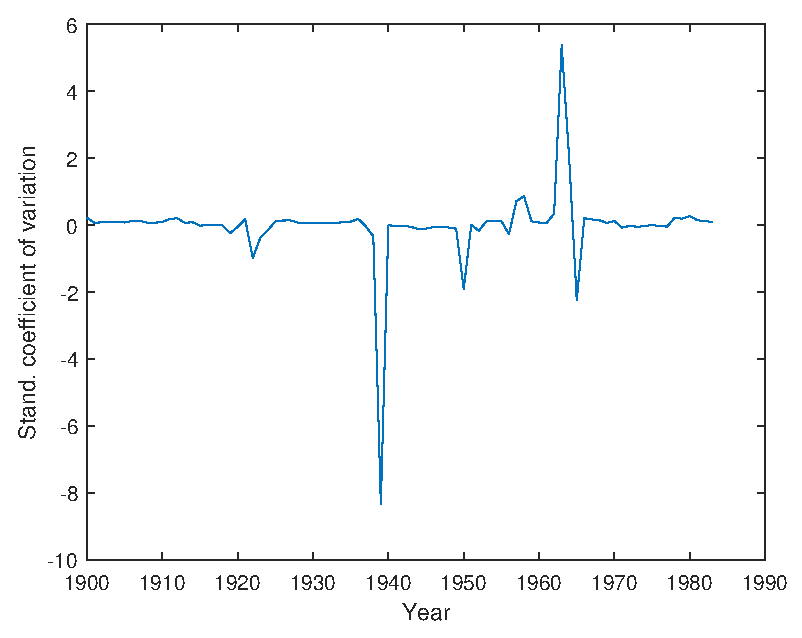
\includegraphics[width = 0.45\textwidth]{Matlab Graphics/Figure_3_1900_1983}
	} &
	\subfloat[Post-1984]{
		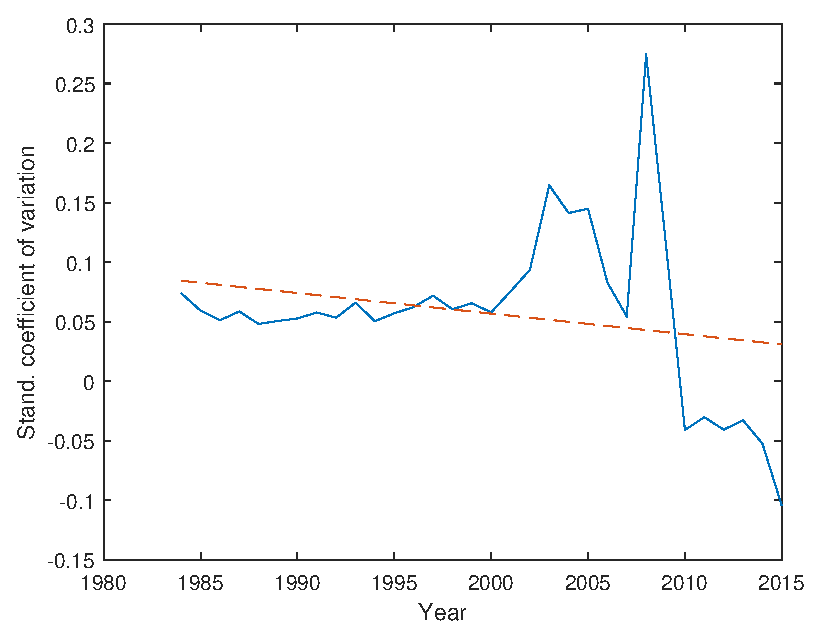
\includegraphics[width = 0.45\textwidth]{Matlab Graphics/Figure_3_1984_2015}
	}\\
	\end{tabular}
	\caption{Standardized coefficient of variation (risk-free rate)}
	\label{fig:stand_coeff_var_riskfree}
\end{figure}

%Major economic shocks such as wartime but also the 1960s posed disturbances to the capital market. Most of the time, however, risk-free rates were rather stable within and across countries. 
The right panel of figure \ref{fig:stand_coeff_var_riskfree} shows a period of global calmness interrupted by the Dot-com bubble and the 2008 financial crisis. Since then risk-free rates entered negative terrain, although monetary authorities' responses were quite consistent in this regard.
Using cross-sectional aggregates it is noteworthy to highlight the two different asset classes' characteristics with respect to ``risk'' and expected return.

\begin{figure}[H]
	\centering
  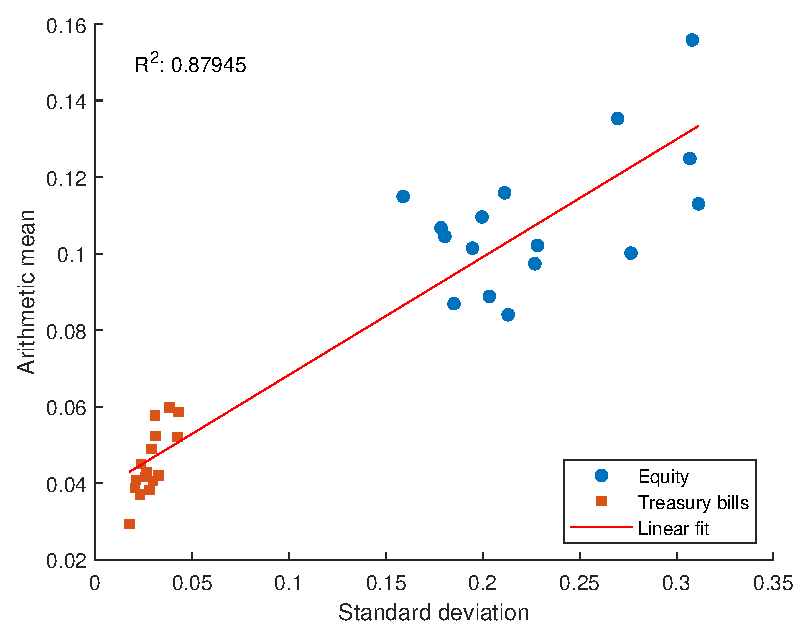
\includegraphics[width=0.7\textwidth]{Matlab Graphics/Figure_4_capital_market_line}
	\caption{Capital market line}
	\label{fig:cml}
\end{figure}

The capital market line (figure \ref{fig:cml}) plots the arithmetic mean of nominal returns against the volatility, measured as the standard deviation of these returns for the two asset classes. Clearly, there is a positive relationship between expected return and volatility within the asset classes but also across them, as confirmed by a formal Chow-test for structural differences between these two classes. Adding an intercept for each class does not improve the goodness of fit (F-distributed Chow-test statistic: 5.42 $<$ critical value with $k=2$ degrees of freedom in the numerator and $n=28$ degrees of freedom in the denominator at $\alpha$ = 0.05: 8.93), hence there are no structural differences in the risk-return relationship across programmes.\\
\\
Finally, turning to the cross-country equity risk premiums reveals dynamic variation within and across countries (figure \ref{fig:erp_countries_time} below).

\begin{figure}[H]
	\centering
  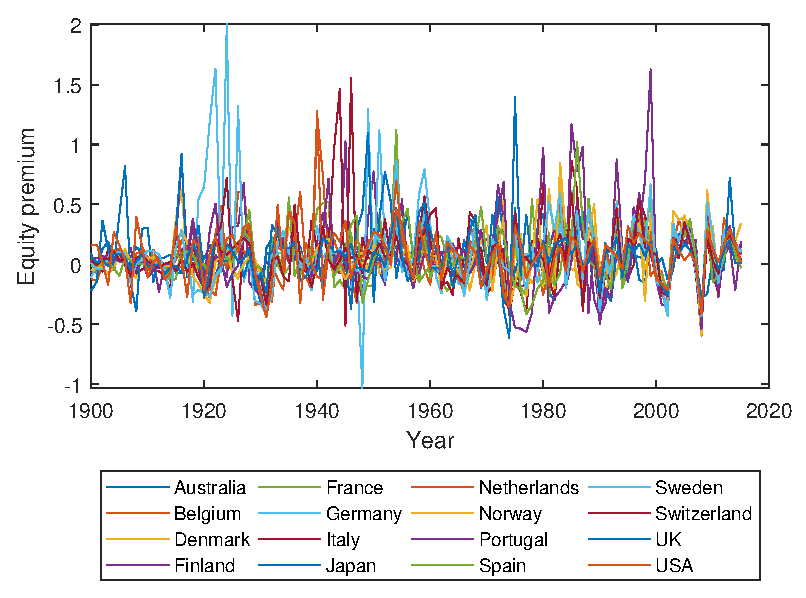
\includegraphics[width=\textwidth]{Matlab Graphics/Figure_5_ERP_countries}
	\caption{Equity risk premiums across countries over time}
	\label{fig:erp_countries_time}
\end{figure}

It appears there is some volatility clustering during wartime across countries but also during prolonged episodes of peace and economic prosperity. The global measure for the equity risk premiums provides more clarity on the dynamic behaviour, that is it's high when there is turmoil and falls as economic conditions improve (see figure \ref{fig:erp_global_time}). 
%A principal component analysis of the ERP cross-country correlations between 1900 and 2015 suggests that one component captures about as much variation as found in six countries (out of sixteen), translating into about 40\% of total variance and appropriately captures within-model (Hotelling's $T^{2}$) and outside-model (squared prediction errors) consistency. Turns out that this component is exactly the negative of the unweighted average. 
%In short, even though cross-country heterogeneity in terms of ERP levels looks pronounced, it actually isn't and only a few exceptional years (see figure \ref{fig:stand_coeff_var_erp}) falling into wartime as well as extraordinary (recovery) growth periods prove the rule. 
Figure \ref{fig:stand_coeff_var_erp} confirms an overall and more recent harmonization \textbf{and} synchronization of equity risk premiums across countries.

\begin{figure}[ht]
	\centering
  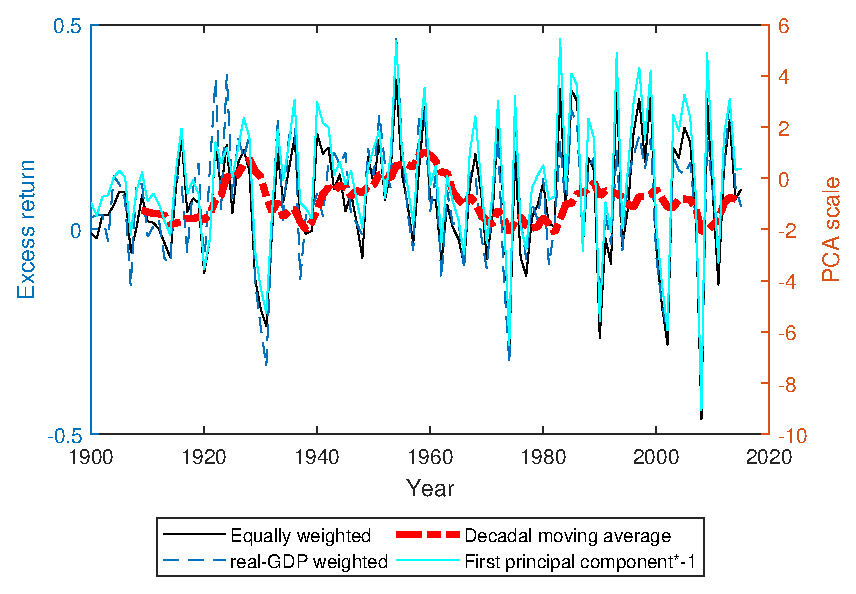
\includegraphics[width=0.8\textwidth]{Matlab Graphics/Figure_6_global_ERP}
	\caption{Global equity risk premium over time}
	\label{fig:erp_global_time}
\end{figure}

\begin{figure}[H]
	\begin{tabular}{cc}
	\subfloat[1900-1983]{
		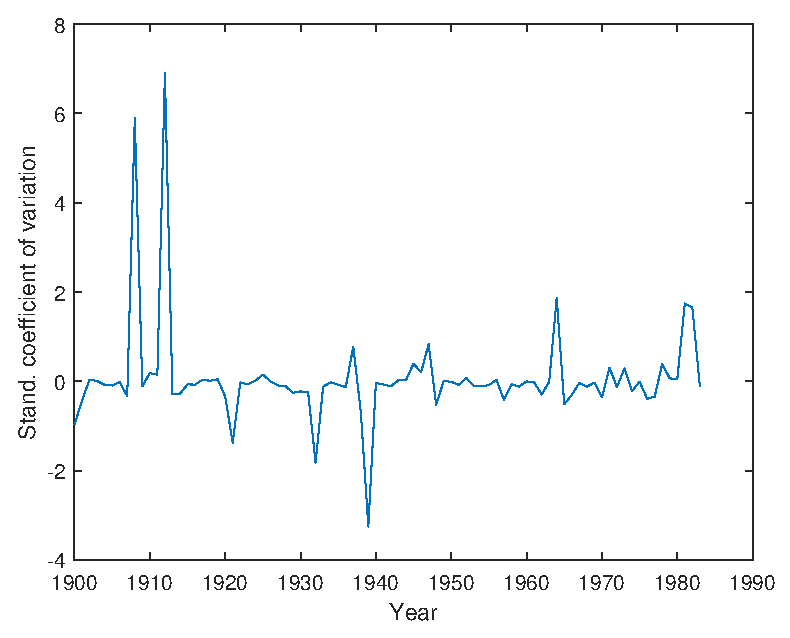
\includegraphics[width = 0.45\textwidth]{Matlab Graphics/Figure_7_1900_1983}
	} &
	\subfloat[Post-1984]{
		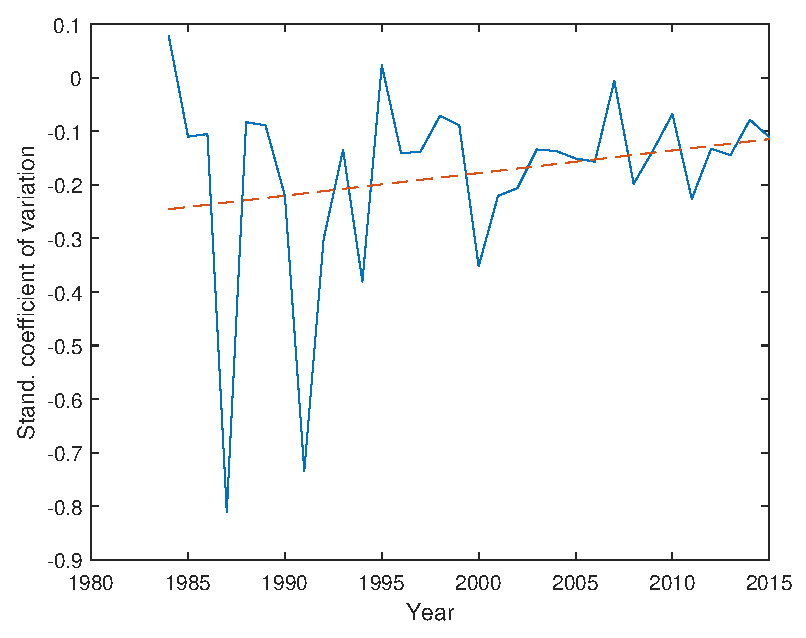
\includegraphics[width = 0.45\textwidth]{Matlab Graphics/Figure_7_1984_2015}
	}\\
	\end{tabular}
	\caption{Standardized coefficient of variation (equity risk premium)}
	\label{fig:stand_coeff_var_erp}
\end{figure}

\newpage
\subsection{International macroeconomic aggregates}
Descriptive statistics for global growth rates are given in table \ref{tab:global_growth} below:

{\renewcommand{\arraystretch}{1.0}
\begin{table}[H]
\begin{center}
\begin{tabular}{rccccc}
\hline
\hline
& \multicolumn{2}{c}{Equally weighted} & & \multicolumn{2}{c}{real GDP-weighted} \\
\cline{2-3} \cline{5-6}
& GDP & consumption & & GDP & consumption\\
\hline
Full sample & & & & &\\
\hline
Mean growth rate p.a. & 2.10 & 1.87 & & 2.14 & 1.81\\
Std.dev. & 2.68 & 2.98 & & 3.12 & 2.53\\
Geometric mean & 2.06 & 1.83 & & 2.09 & 1.78\\
Median & 2.41 & 1.91 & & 2.24 & 2.03\\
Max & 11.10 & 15.17 & & 9.60 & 13.84\\
Min & -6.40 & -6.98 & & -9.41 & -5.28\\
Kurtosis & 5.00 & 8.02 & & 5.15 & 7.45\\
\hline
Post-1984 & & & & &\\
\hline
Mean growth rate p.a. & 1.60 & 1.53 & & 1.67 & 1.71\\
Std.dev. & 1.60 & 1.23 & & 1.54 & 1.18\\
Geometric mean & 1.59 & 1.52 & & 1.66 & 1.71\\
Median & 2.02 & 1.66 & & 1.94 & 1.75\\
Max & 3.66 & 3.60 & & 4.19 & 3.55\\
Min & -4.38 & -1.54 & & -4.20 & -1.45\\
Kurtosis & 7.92 & 2.96 & & 8.99 & 3.52\\
\hline
\hline
\end{tabular} 
\end{center}
\caption{Global growth rates (1900-2015), \%}
\label{tab:global_growth}
\end{table}

As one can see, GDP growth was higher than consumption growth and slightly more volatile. 
%Both macroeconomic aggregate's growth rates are centered around their mean values with rates ranging from -6.98\% to 15.17\% for consumption when all countries were equally weighted and from -9.41\% in GDP to 13.84\% in consumption when countries were real-GDP weighted. 
The post-1984 period is characterised by overall lower growth rates but also volatility where consumption growth is nearly normal distributed. Table \ref{tab:global_growth_HP} in the appendix presents the same statistics for growth rates of the HP-filtered trend component where growth rates are overall lower and also less volatile than the unfiltered data.


Growth rates across countries are presented in table \ref{tab:real_growth_countries} below. 
{\renewcommand{\arraystretch}{1.0}
\begin{table}[H]
\begin{center}
\begin{tabular}{rccccccccccc}
\hline
\hline
Country & \multicolumn{5}{c}{Full sample (1870-2015)} & & \multicolumn{5}{c}{post-1984} \\
%\cline{2-6} \cline{8-12}
\hline
 & \multicolumn{2}{c}{GDP} & & \multicolumn{2}{c}{consumption} & & \multicolumn{2}{c}{GDP} & & \multicolumn{2}{c}{Consumption}\\
\cline{2-3} \cline{5-6} \cline{8-9} \cline{11-12}
 & Mean & Std & & Mean & Std & & Mean & Std & & Mean & Std\\
\hline
Australia & 1.54 & 4.10 & & 1.28 & 5.73 & & 1.91 & 1.47 & & 1.77 & 1.39\\
Belgium$^{*}$ & 1.93 & 8.16 & & 1.73 & 8.64 & & 1.49 & 1.50 & & 1.22 & 1.26 \\
Denmark & 1.76 & 3.66 & & 1.53 & 5.27 & & 1.17 & 1.95 & & 0.93 & 2.40 \\
Finland & 2.18 & 4.50 & & 2.24 & 5.51 & & 1.52 & 3.40 & & 1.84 & 2.82\\
France & 1.85 & 6.25 & & 1.60 & 6.53 & & 1.26 & 1.46 & & 1.25 & 1.18\\
Germany & 2.09 & 7.92 & & 1.84 & 5.54 & & 1.70 & 1.97 & & 1.40 & 1.22\\
Italy & 1.92 & 4.68 & & 1.55 & 3.70 & & 1.37 & 2.60 & & 0.96 & 2.29\\
Japan$^{*}$ & 2.62 & 5.97 & & 2.36 & 6.70 & & 1.55 & 2.23 & & 1.61 & 1.52\\
Netherlands & 1.79 & 7.38 & & 1.76 & 8.32 & & 1.73 & 1.76 & & 1.15 & 1.66 \\
Norway & 2.18 & 3.56 & & 1.92 & 3.71 & & 1.83 & 1.95 & & 2.27 & 2.32\\
Portugal$^{*}$ & 1.95 & 4.25 & & 2.49 & 4.42 & & 1.77 & 2.85 & & 2.31 & 3.21 \\
Spain & 2.00 & 4.90 & & 1.88 &  7.53 & & 2.04 & 2.67 & & 1.55 & 2.71\\
Sweden & 2.10 & 3.39 & & 1.91 & 4.33 & & 1.66 & 2.42 & & 1.35 & 2.03\\
Switzerland & 1.50 & 3.90 & & 1.40 & 6.03 & & 1.03 & 1.69 & & 0.84 & 0.86\\
United Kingdom & 1.45 & 2.87 & & 1.37 & 2.80 & & 1.80 & 1.88 & & 2.10 & 2.25\\
United States & 2.05 & 4.90 & & 1.83 & 3.48 & & 1.73 & 1.75 & & 1.95 & 1.45 \\
\hline
Average & 1.93 & - & & 1.79 & - & & 1.60 & - & & 1.53 & -\\

\hline
\hline
\multicolumn{12}{c}{$^{*}$ Belgium: 1914-2015, Japan: 1875-2015, Portugal: 1911-2015}
\end{tabular} 
\end{center}
\caption{Real growth rates (country-level), \%}
\label{tab:real_growth_countries}
\end{table}

Table \ref{tab:real_growth_countries_HP} in the appendix repeats the same exercise with HP-trend filtered data\footnote{Individual country's indices for real GDP per capita and real consumption expenditures per capita were HP-filtered first and the growth rates of the trend component were then real GDP-weighted.} with overall lower growth rates and lower volatility.

\begin{figure}[H]
	\begin{tabular}{cc}
	\subfloat[Real GDP/capita growth]{
		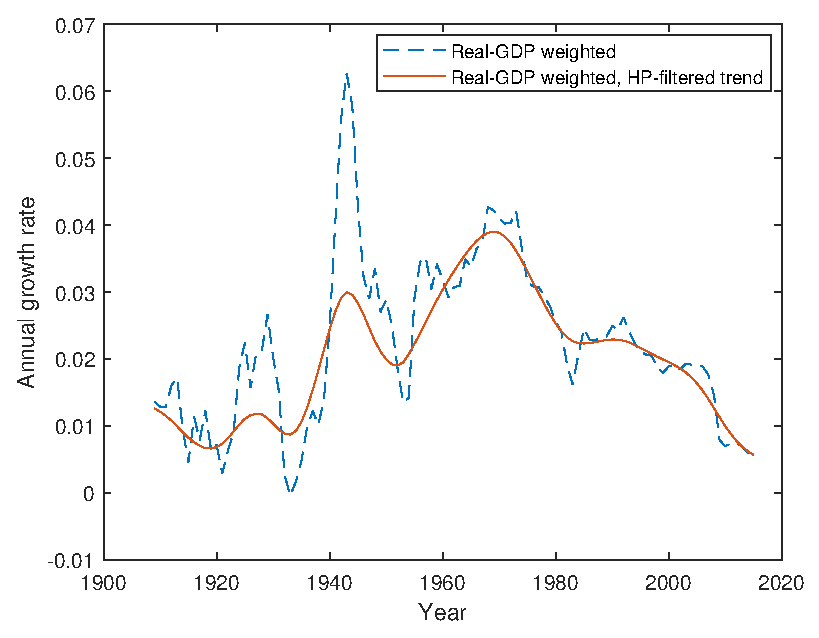
\includegraphics[width = 0.45\textwidth]{Matlab Graphics/Figure_8_GDP}
	} &
	\subfloat[Real consumption/capita growth]{
		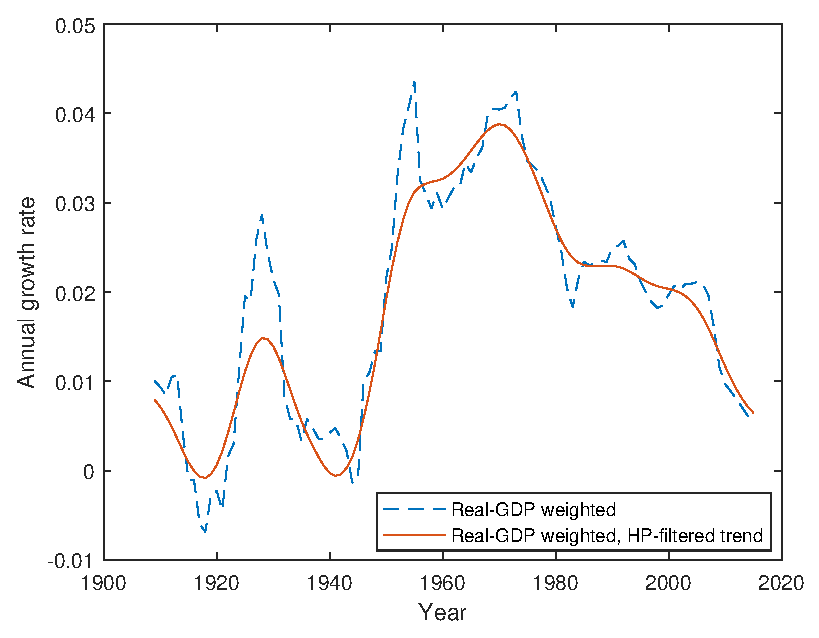
\includegraphics[width = 0.45\textwidth]{Matlab Graphics/Figure_8_cons}
	}\\
	\end{tabular}
	\caption{Decadal moving averages of real-GDP weighted growth rates}
	\label{fig:10y_MA_weighted_growth}
\end{figure}

Figure \ref{fig:10y_MA_weighted_growth} shows the 10-year moving averages for the annual growth rates together with the HP-filtered trend components' growth rates per country, all real-GDP weighted. Since the 1970s both macroeconomic aggregates have been growing at positive but decreasing rates where GDP appears to fluctuate more frequently and variably than consumption. 
Finally, figure \ref{fig:global_business_cycle} displays the real-GDP weighted, HP-filtered countries' trend components growth capturing the world's business cycle dynamics of the last century. Since the 1960s both aggregates move in almost perfect tandem following a downward trend from 4\% annual growth to less than 1\% per year.

\begin{figure}[H]
	\centering
  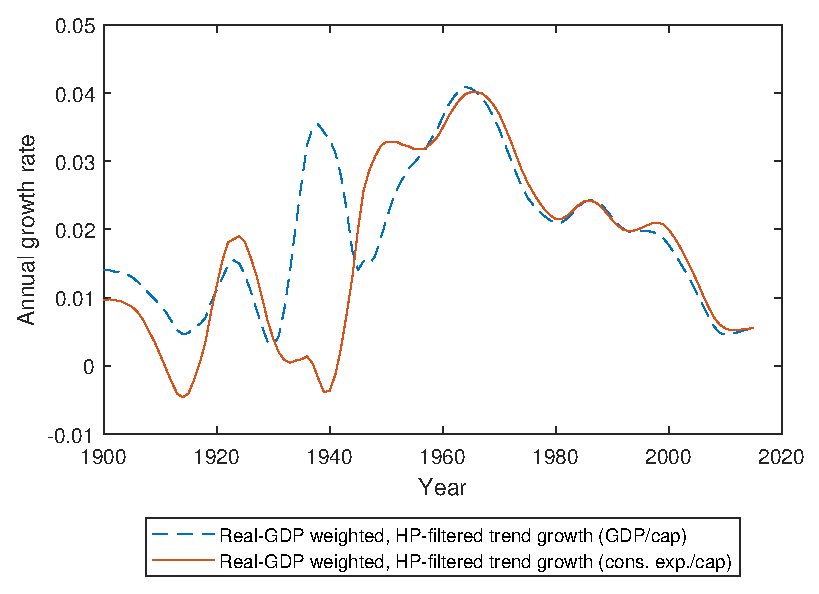
\includegraphics[width=\textwidth]{Matlab Graphics/Figure_9}
	\caption{Global business cycle}
	\label{fig:global_business_cycle}
\end{figure}

\subsection{Macro-finance}
According to \citet{Cochrane2017}, ``Macro-finance studies the relationship between asset prices and economic fluctuations.'' Stock market returns driven by capital gains tend to be high during economic expansions, reflecting higher expected corporate earnings are low during recessions. ``The'' interest rate (solid red line in figure \ref{fig:financial_aggregates_cycles}), however, reflects the opportunity cost of consuming rather than investing and provides a, perhaps the most decisive, incentive to postpone consumption (solid blue line in figure \ref{fig:financial_aggregates_cycles}) when it's high, resulting in lower consumption growth. Figure \ref{fig:financial_aggregates_cycles} below illustrates these relationships of real-GDP weighted returns and growth rates. 
\begin{figure}[ht]
	\centering
  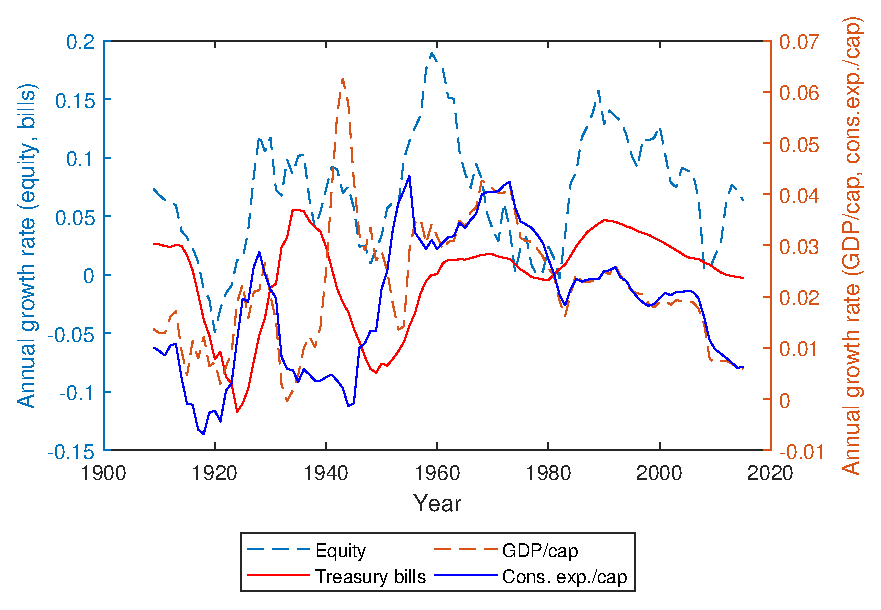
\includegraphics[width=0.8\textwidth]{Matlab Graphics/Figure_10}
	\caption{Financial markets and real economy}
	\label{fig:financial_aggregates_cycles}
\end{figure}
Whereas the first fact, i.e. there is a positive correlation between GDP growth (or consumption growth) and stock market returns ($\rho_{(r^{e}, \Delta GDP)} = 0.23$, $\rho_{(r^{e}, \Delta cons)} = 0.35$) roughly holds over a long horizon the second relationship, i.e. a negative correlation between GDP growth (or consumption growth) and the interest rate appears to have broken down since the 1960s (pre-1965: $\rho_{(r^{f}, \Delta GDP)} = -0.16$, $\rho_{(r^{f}, \Delta cons)} = -0.17$, post-1965: $\rho_{(r^{f}, \Delta GDP)} = 0.09$, $\rho_{(r^{f}, \Delta cons)} = 0.03$). These covariances are exactly the quantities of undiversifyable risk that investors, in theory, are compensated for. The \textit{adequate} magnitude in expectation is the equity risk premium which has been measured in a vast body of literature and applications between 4\% and 8\%.

%Going back to the last relationship between (expected) excess return, risk aversion and variance in consumption growth in subsection \ref{Power utility} clearly illustrates this link. 
For any given level of risk aversion, higher variability in consumption growth (i.e. risk) increases the expected excess return by decreasing the risk-free rate due to the precautionary savings effect. Figure \ref{fig:ERP_riskfree_volatility} below illustrates the theoretical conjectures in the data with the aforementioned divergence starting in the 1980s when global interest rates started to descend.
\begin{figure}[H]
	\begin{tabular}{cc}
	\subfloat[Equity risk premium and consumption volatility]{
		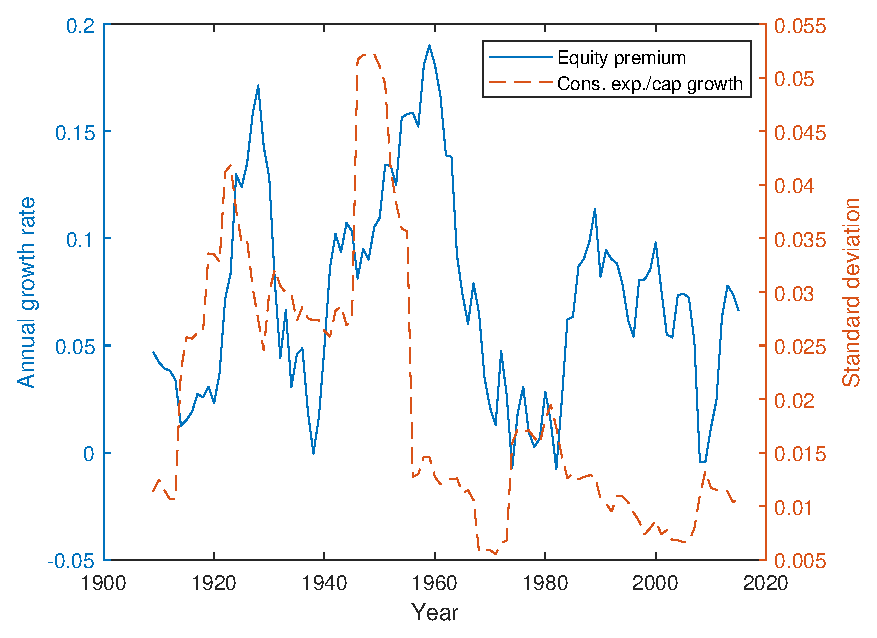
\includegraphics[width = 0.45\textwidth]{Matlab Graphics/Figure_11_ERP}
	} &
	\subfloat[Risk-free rate and consumption volatility]{
		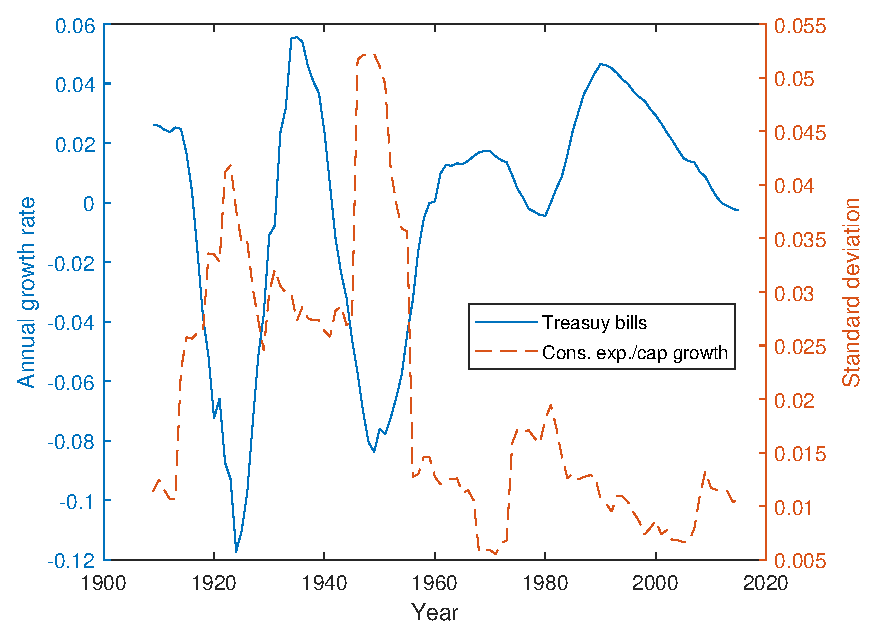
\includegraphics[width = 0.45\textwidth]{Matlab Graphics/Figure_11_riskfree}
	}\\
	\end{tabular}
	\caption{Global decadal moving average of ERP and standard deviation of consumption growth, real-GDP weighted}
	\label{fig:ERP_riskfree_volatility}
\end{figure}
The ERP is positively correlated with the variability in consumption growth (Pearson correlation coefficient of 0.22) whereas the risk-free rate is strongly negatively correlated with variability in consumption growth (Pearson correlation coefficient of -0.73).


With all the ingredients from a (log-normal) consumption-based asset pricing model under time-separable expected utility at hand it is straightforward to derive implied coefficients of relative risk aversion \underline{$\gamma$} (see tables \ref{tab:results_consumption} and \ref{tab:results_GDP} for consumption data and GDP data, respectively for comparison).
%As countries exhibit heterogeneity in risk premiums and consumption growth moments so they do in implied preferences. Most importantly, the implied coefficients of relative risk aversion range from 8 (Belgium) to a whopping 76 (United Kingdom)! 
These are orders of magnitude above the standard evidence for low values of $\gamma$, around 1, coming from the relationship between the risk-free rate and consumption growth which rises quickly in $\gamma$.

\subsection{Disaster empirics}
%What exactly defines an economic disaster? In general, it is a state of very low consumption growth and hence high marginal utility of consumption. Such state must be distinctively different and much more `painful' than normal economic fluctuations which can extend to externality effects such as the destruction of intangible capital. Extreme one-period contractions alone might not capture a disastrous event as severe recessions are usually characterized by prolonged periods of economic decline.

A somewhat arbitrary lower bound \cite{Barro2006} needs to be chosen that would at least approximately match the proportionate decline required to materialize the extremely high level of marginal utility. In the baseline calibration I follow \citet{Barro2012} and set the threshold to 0.095, i.e. a contraction of at least 9.5\%. This threshold corresponds to the 92$^{nd}$ percentile of the left-sided distribution of all annual growth rates of GDP and consumption for the entire sample. Anything above this proportionate decline is considered a `disaster' which is the case for about 8\% of the time in annual growth rates in the full sample.
A disastrous event may occur as period of successive economic decline. I apply a NBER-like peak-to-trough procedure (see Python code \ref{lst:code} in the appendix) to identify those periods and occurrences. Figure \ref{fig:US_cons_disaster} below illustrates the identified disaster periods (grey) with respect to consumption growth. 

\begin{figure}[H]
	\centering
  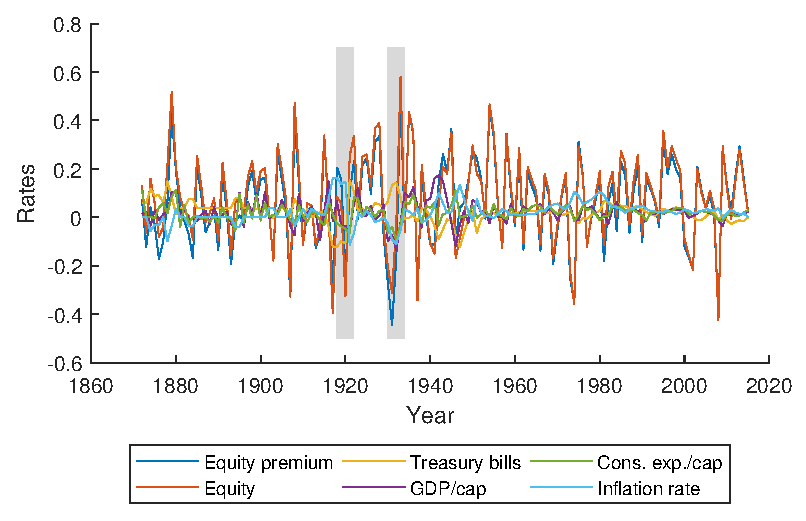
\includegraphics[width=\textwidth]{Matlab Graphics/Cons_disaster_US}
	\caption{US, consumption disasters}
	\label{fig:US_cons_disaster}
\end{figure}

For the US there were two disaster periods of equal lengths but different contraction sizes identified: the first one started 1918 with the onset of a global pandemic caused by an H1N1 virus, better known as the Spanish flu, which would later account for 500 million deaths worldwide and about 675,000 deaths occurring in the United States and triggered a depression in subsequent years lasting for four years (until 1922) with an average proportionate contraction of 18\%. The second consumption disaster period started in 1930 and captures the most severe part of the Great Depression where real consumption per capita fell about 23\% per year over this period (ended in 1934) (see \citet{Nakamura2013} for similar estimates).\\

The disaster probability $p$ is calculated as the total number of disasters (irrespective of duration) divided by the number of non-disaster years to provide a measure at an annual frequency. The expected disaster size $\mathop{\mathbb{E}}(b)$ is the unweighted average of annual proportionate declines > threshold.\\

{\renewcommand{\arraystretch}{1}
\begin{table}[H]
\begin{center}
\begin{tabular}{rccccc}
\hline
\hline
\multirow{3}{*}{Country} & \multirow{3}{*}{\shortstack{No.\\disasters}} & \multirow{3}{*}{\shortstack{No.\\disaster\\years}} & \multirow{3}{*}{\shortstack{No. non-\\disaster\\years}} & \multirow{3}{*}{\shortstack{Disaster\\probability\\(\%)}} & \multirow{3}{*}{\shortstack{Average\\disaster size\\(\%)}}\\
& & & & &\\
& & & & &\\
\hline
Australia & 6 & 17 & 128 & 4.69 & 22.60\\
Belgium$^{*}$ & 4 & 11 & 91 & 4.40 & 34.50\\
Denmark & 3 & 6 & 139 & 2.16 & 22.31\\
Finland & 5 & 16 & 129 & 3.90 & 21.75\\
France & 2 & 8 & 137 & 1.50 & 49.83\\
Germany & 4 & 17 & 128 & 3.13 & 31.75\\
Italy & 1 & 5 & 140 & 0.71 & 32.13\\
Japan$^{*}$ & 1 & 8 & 133 & 0.75 & 90.35\\
Netherlands & 3 & 10 & 135 & 2.22 & 42.14\\
Norway & 3 & 9 & 136 & 2.21 & 14.69\\
Portugal$^{*}$ & 3 & 9 & 96 & 3.13 & 15.25\\
Spain & 13 & 31 & 114 & 11.40 & 16.21\\
Sweden & 2 & 4 & 141 & 1.41 & 14.82\\
Switzerland & 6 & 14 & 131 & 4.60 & 17.73\\
United Kingdom & 2 & 8 & 137 & 1.50 & 17.72\\
United States & 2 & 8 & 137 & 1.50 & 20.02\\
\hline
$\Sigma$ & 60 & 181 & 2,052 & 2.92 & $\mu=28.99$\\
\hline
\hline
\multicolumn{6}{c}{$^{*}$ Belgium: 1914-2015, Japan: 1875-2015, Portugal: 1911-2015}
\end{tabular} 
\end{center}
\caption{Disaster risk moments (consumption)}
\label{tab:disaster_risk_consumption}
\end{table}

As table \ref{tab:disaster_risk_consumption} amd figure \ref{fig:Gant_consumption} show there is quite some variation across countries in propensity with respect to consumption disasters. 

\begin{figure}[H]
	\centering
  \includegraphics[width=\textwidth]{Graphics/Gantt_consumption_highres.PNG}
	\caption{Consumption disasters across countries over time}
	\label{fig:Gant_consumption}
\end{figure}

Clearly, wartime events affected most countries, though with different strength. Spain experienced multiple rather mild disasters whereas France, the Netherlands and Japan were hit by only few but abysmal events. The interactive version with additional information on individual disasters can be accessed from this \textcolor{blue}{\href{https://plotly.com/~gerwolf/54/consumption-disasters-percentage/}{link}}:\\
(https://plotly.com/~gerwolf/54/consumption-disasters-percentage/)
\\
Table \ref{tab:disaster_risk_gdp} and figure \ref{fig:Gant_GDP} in the appendix provide the same overview for GDP data. [\textcolor{blue}{\href{https://plotly.com/~gerwolf/68/gdp-disasters-percentage/}{Interactive version}}:\\
(https://plotly.com/~gerwolf/68/gdp-disasters-percentage/)]
\\
\\Consumption disasters occur slightly more frequently than GDP disasters but with a larger average contraction size. Notably, Japan suffered from the worst consumption disasters in the data set in the wake of WWII whereas the GDP contractions were not as severe. In general, average GDP contractions were less pronounced than consumption contractions which is probably due to the stabilizing measures taken by authorities by the onset of a disaster. Moreover, consumption tends to continue falling in response to a disaster shock before recovering, resulting in longer disaster durations pointing towards the crucial role of the IES and a high consumers' willingness to substitute consumption across time.







~\\
\section{Results} \label{Results}

\subsection{Baseline calibration} \label{Baseline calibration}

The disaster risk model was fully calibrated except for values of $\beta$ (or $\rho$) where $\beta = \frac{1}{1+\rho}$ which was set to 0.95, corresponding to an annualized, hypothetical risk-free interest rate ``if consumption were known to be constant forever at its current level, with no growth and no volatility'' \cite{Constantinides2003} of 5\%\footnote{5\% is approximately the annual, unweighted average of nominal T-bills and bonds in \citet{Jorda2017} across countries in the sample and was also used by \citet{Weil1989} for calibration that resulted in the \textit{risk-free rate puzzle}} and the IES which was set to the value of microeconometric evidence from cross-individual differences in after-tax real interest rates of (around) 2 \cite{Gruber2013}. Table \ref{tab:growth_non_disaster} in the appendix provides additional moments used for calibration of exogeneous productivity growth and variability during non-disaster periods.

Solving the non-linear equation for the ERP incorporating disaster risk with \texttt{MINPACK}'s \texttt{hybrd} subroutine implemented in Python yielded the implied coefficients of relative risk aversion $\boldsymbol{\gamma}$. For comparison the implied coefficients of relative risk aversion from the original specification leading to the puzzle indicated with an upper bar are also presented in table \ref{tab:results_consumption} below.\\

{\renewcommand{\arraystretch}{1.0}
\begin{table}[!ht]
\begin{center}
\begin{tabular}{rccccccc}
\hline
\hline
Country & $g^{*}$ (\%) & $\rho^{*}$ & $\beta^{*}$ & $r^{e}$ (\%) & $r^{f}$ (\%) & \underline{$\gamma$} & \boldsymbol{$\gamma$}\\
\hline

Australia & 1.55 & 0.0628 & 0.9409 & 6.91 & 2.52 & 20.10 & 5.54\\ 

Belgium & 2.14 & 0.0419 & 0.9598 & 7.14 & 3.20 & 7.91 &  2.54\\ 

Denmark & 1.69 & 0.0308 & 0.9701 & 6.77 & 3.50 & 17.66 &  6.53\\ 

Finland & 2.61 & 0.0444 & 0.9575 & 7.82 & 0.92 & 34.01 &  8.15\\ 

France & 1.82 & 0.0405 & 0.9610 & 6.70 & 3.81 & 10.17 &  2.07\\ 

Germany & 2.17 & 0.0622 & 0.9415 & 7.54 & 0.56 & 34.08 &  5.13\\ 

Italy & 1.66 & 0.0310 & 0.9700 & 6.76 & 2.43 & 47.37 &  7.21\\ 

Japan & 2.65 & 0.0456 & 0.9564 & 7.20 & 1.01 & 20.62 &  0.97\\ 

Netherlands & 2.12 & 0.0429 & 0.9588 & 7.16 & 2.82 & 9.41 &  2.66\\ 

Norway & 2.09 & -0.0426 & 1.0445 & 6.96 & 3.63 & 36.28 &  12.67\\ 

Portugal & 2.79 & -0.0777 & 1.0843 & 7.25 & 4.49 & 21.17 &  8.61\\ 

Spain & 2.54 & 0.0226 & 0.9780 & 7.47 & 3.23 & 11.23 &  5.09\\ 

Sweden & 2.04 & 0.0159 & 0.9843 & 7.18 & 2.88 & 34.45 &  14.48\\ 

Switzerland & 1.69 & 0.0519 & 0.9507 & 6.94 & 3.10 & 15.88 &  6.49\\ 

United Kingdom & 1.48 & 0.0290 & 0.9718 & 6.65 & 2.69 & 76.32 &  13.36\\ 

United States & 1.98 & -0.0028 & 1.0028 & 6.98 & 2.80 & 51.76 &  11.01\\
\hline
Global & & & & & & &\\
\hline 
\hline
\end{tabular} 
\end{center}
\caption{Calibration \& results (consumption)}
\label{tab:results_consumption}
\end{table}
The results for GDP data are documented in table \ref{tab:results_GDP} in the appendix. A few observations can be made from these results:
\begin{enumerate}
    \item When accounting for disaster risk \textbf{all} implied coefficients of relative risk aversion decrease. For consumption (GDP) data the implied coefficients drop by 72\% (69\%) on average compared to the benchmark values.
    \item The relative order is approximately preserved, meaning that the disaster risk model is consistent when accounting for heterogeneity in disaster characteristics (see figure \ref{fig:disaster_vs_benchmark_gamma}).
    \item Risk-free rates are consistently overestimated. They are, nevertheless roughly in line with the levels of their empirical counterparts and this relationship is statistically significant at the 0.05 confidence level (see figures \ref{fig:actual_vs_predicted_rates_cons} and \ref{fig:actual_vs_predicted_rates_GDP} [appendix] for consumption and GDP data, respectively). However, predicted risk-free rates are upwards biased (also statistically significant mean of residuals, $\mu^{cons} = -2.54$, $\mu^{GDP} = -2.62$) and are never negative whereas long-run real T-bill rates were negative for six countries in the sample.
    \item For consumption (GDP) data two (six) countries have negative implied effective time preference rates $\rho^{*}$, meaning that $\beta^{*} > 1$ when assuming that markets are complete, i.e. $(1+r^{*})\beta^{*} = 1$ and $r^{*} = \rho^{*}$ in the steady state. From a mathematical point of view this may be problematic: the infinite, discounted sum of expected utility explodes as $t \longrightarrow \infty$. Intuitively, agents prefer present utility over utility in the future due to \textit{impatience}. This presumption translates into a positive interest rate. If this wasn't the case agents would have an incentive to borrow an infinite amount and the transversality condition would be violated which cannot coincide with a competitive equilibrium. However, \citet{Kocherlakota1990} argues that a parameterized version of the subject discount factor (such as $\beta^{*}$) greater than 1 can indeed coincide with a competitive equilibrium in a growth environment, given that a) the IES is less than 1 and the stream of consumption is constant. Under these conditions the agent prefers future consumption over present consumption which conflicts with the empirical observation that real interest rates are typically positive. In the sample presented in chapter \ref{Data}, however, seven countries appeared to have negative real T-bills rates whereas the model predicted strictly positive risk-free rates. Of those seven countries three implied negative effective time preference rates $\rho^{*}$ when using GDP data. Also, \citet{Hansen1982} derived point estimates of $\beta$ significantly greater than 1, adding support that in artificial economies ``unreasonable'' \cite{Kocherlakota1990} values for $\beta > 1$ shouldn't be precluded.
    \item In general, when moving from GDP data to consumption data four out of six countries' effective subjective discount factors $\beta^{*}$ become less than 1, indicating that consumption is a more robust measure with respect to intertemporal considerations than overall output. Effective time preference rates, however, behave inconsistently when using consumption and GDP data, meaning that for one country (Norway) $\beta^{*}$ gets closer to 1 (from GDP to consumption) whereas for the other country (Portugal) $\beta^{*}$ moves further away from 1. 
    \item The implied coefficients of relative risk aversion are somewhat higher when using GDP data compared to consumption data. Levels of the predicted rates are also higher, shifted by a constant that is due to the effect of the product of lower disaster probability and average disaster size which more than outweighs the higher average growth rates and higher variability in growth rates in non-disaster years.
\end{enumerate}

\begin{figure}[H]
	\begin{tabular}{cc}
	\subfloat[Consumption data implied $\gamma$]{
		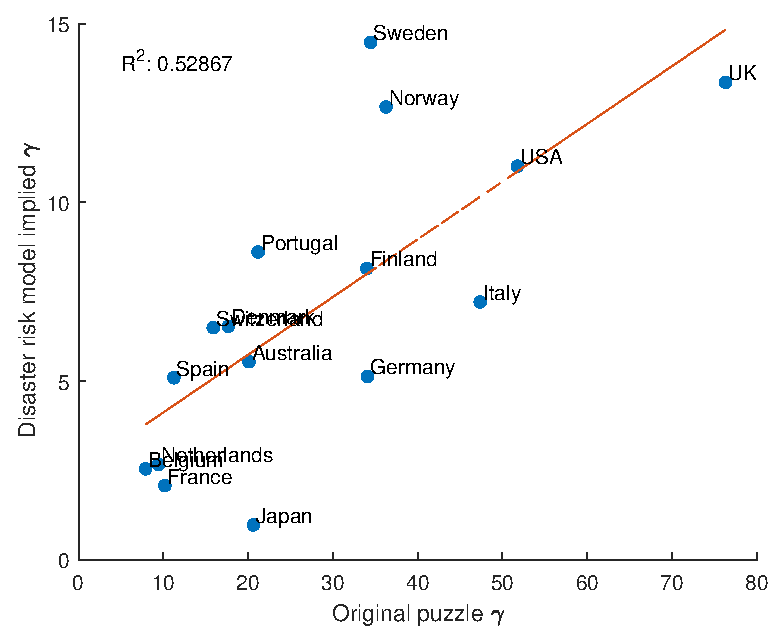
\includegraphics[width = 0.45\textwidth]{Matlab Graphics/Reduction_gamma_cons}
	} &
	\subfloat[GDP-data implied $\gamma$]{
		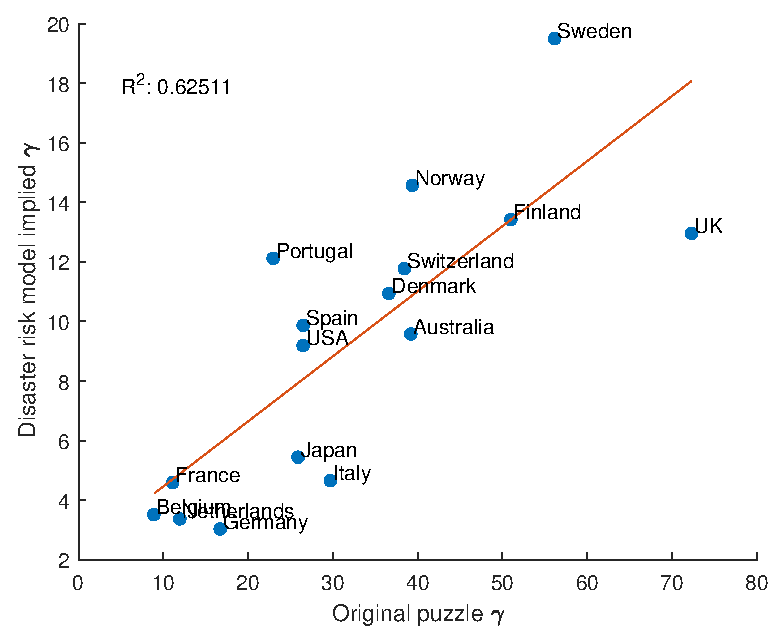
\includegraphics[width = 0.45\textwidth]{Matlab Graphics/Reduction_gamma_GDP}
	}\\
	\end{tabular}
	\caption{Disaster model $\gamma$ vs. benchmark model $\gamma$}
	\label{fig:disaster_vs_benchmark_gamma}
\end{figure}


\begin{figure}[H]
	\begin{tabular}{cc}
	\subfloat[Expected rates of return on equity]{
		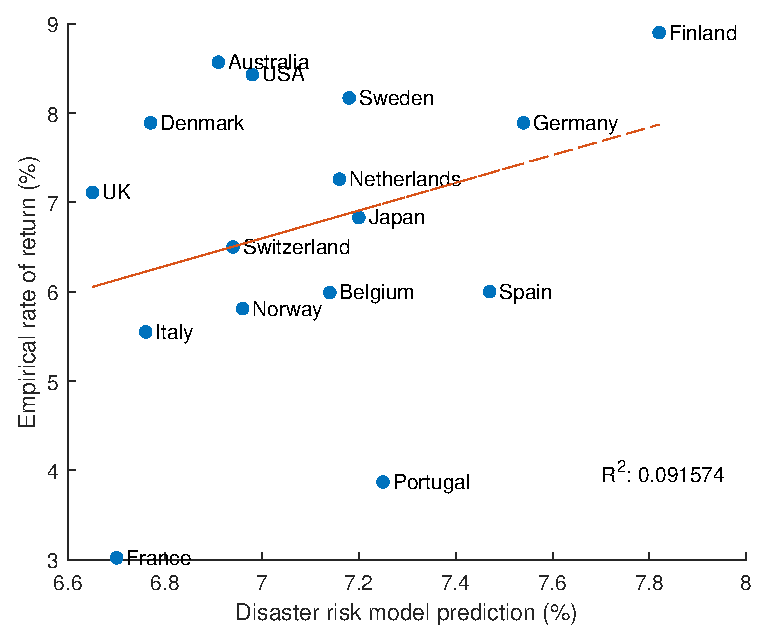
\includegraphics[width = 0.45\textwidth]{Matlab Graphics/Actual_vs_predicted_equity_cons}
	} &
	\subfloat[Risk-free rates]{
		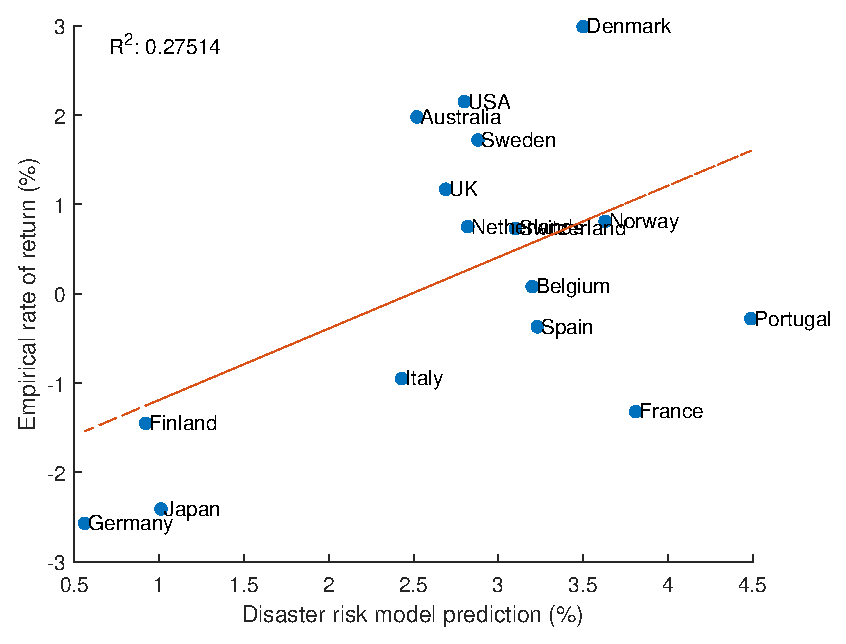
\includegraphics[width = 0.45\textwidth]{Matlab Graphics/Actual_vs_predicted_riskfree_cons}
	}\\
	\end{tabular}
	\caption{Actual vs. predicted rates of return (consumption data)}
	\label{fig:actual_vs_predicted_rates_cons}
\end{figure}


\subsection{Robustness} \label{Robustness}

As already mentioned the disaster threshold was chosen arbitrarily, thus verifying robustness of the results when varying that parameter seems appropriate. When increasing the threshold from a proportionate decline of 9.5\% to 15\% (see table \ref{tab:disaster_risk_threshold} in the appendix) the total number of disaster events in the sample decreases from 60 to 40 and from 56 to 32 for consumption data and GDP data, respectively. 

{\renewcommand{\arraystretch}{1}
\begin{table}[p]
\begin{center}
\begin{tabular}{rccccccc}
\hline
\hline
Country & $g^{*}$ (\%) & $\rho^{*}$ & $\beta^{*}$ & $r^{e}$ (\%) & $r^{f}$ (\%) & \underline{$\gamma$} & \boldsymbol{$\gamma$}\\
\hline
\multicolumn{8}{c}{Consumption}\\
\hline

Australia & 1.55 & 0.0628 & 0.9409 & 6.91 & 2.52 & 20.10 & 5.54\\ 

Belgium & 2.08 & 0.0438 & 0.9580 & 7.07 & 3.13 & 7.91 &  2.11\\ 

Denmark & 1.67 & 0.0311 & 0.9698 & 6.75 & 3.48 & 17.66 &  6.11\\ 

Finland & 2.51 & 0.0425 & 0.9593 & 7.69 & 0.80 & 34.01 &  7.00\\ 

France & 1.82 & 0.0405 & 0.9610 & 6.70 & 3.81 & 10.17 &  2.07\\ 

Germany & 2.11 & 0.0515 & 0.9510 & 7.35 & 0.37 & 34.08 &  3.14\\ 

Italy & 1.66 & 0.0310 & 0.9700 & 6.80 & 2.43 & 47.37 &  7.21\\ 

Japan & 2.65 & 0.0456 & 0.9564 & 7.17 & 1.01 & 20.62 &  0.97\\ 

Netherlands & 2.12 & 0.0429 & 0.9588 & 7.16 & 2.82 & 9.41 &  2.66\\ 

Norway & 2.02 & -0.0358 & 1.0371 & 6.91 & 3.58 & 36.28 &  12.30\\ 

Portugal & 2.70 & -0.0564 & 1.0598 & 7.17 & 4.41 & 21.17 &  7.41\\ 

Spain & 2.31 & 0.0326 & 0.9684 & 7.33 & 3.08 & 11.23 &  4.61\\ 

Sweden & 2.04 & 0.0186 & 0.9818 & 7.18 & 2.89 & 34.45 &  15.05\\ 

Switzerland & 1.67 & 0.0532 & 0.9495 & 6.94 & 3.10 & 15.88 &  6.55\\ 

United Kingdom & 1.48 & 0.0290 & 0.9718 & 6.65 & 2.69 & 76.32 &  13.36\\ 

United States & 1.98 & -0.0028 & 1.0028 & 6.98 & 2.80 & 51.76 &  11.01\\
\hline
Global & & & & & & &\\
\hline
 & & & & & \\
  & & & & & \\
\hline
\multicolumn{8}{c}{GDP}\\
\hline
Australia & 1.71 & 0.0429 & 0.9589 & 6.92 & 2.53 & 39.18 & 9.20\\ 

Belgium & 2.30 & 0.0346 & 0.9665 & 7.25 & 3.31 & 8.88 &  3.32\\ 

Denmark & 1.84 & -0.0082 & 1.0083 & 6.74 & 3.48 & 36.61 &  9.00\\ 

Finland & 2.29 & 0.0317 & 0.9692 & 7.43 & 0.54 & 50.99 &  9.23\\ 

France & 2.14 & 0.0162 & 0.9840 & 6.96 & 4.07 & 11.10 &  4.60\\ 

Germany & 2.40 & 0.0482 & 0.9540 & 7.54 & 0.56 & 16.70 &  2.36\\ 

Italy & 2.10 & 0.0248 & 0.9758 & 7.03 & 2.70 & 29.69 &  4.65\\ 

Japan & 2.85 & 0.0250 & 0.9756 & 7.50 & 1.34 & 25.89 &  2.78\\ 

Netherlands & 2.14 & 0.0403 & 0.9612 & 7.12 & 2.78 & 11.94 &  2.70\\ 

Norway & 2.27 & -0.0919 & 1.1012 & 7.07 & 3.74 & 39.36 &  16.23\\ 

Portugal & 2.06 & -0.0400 & 1.0417 & 6.92 & 4.16 & 22.95 &  12.11\\ 

Spain & 2.14 & 0.0100 & 0.9901 & 7.05 & 2.81 & 26.49 &  6.62\\ 

Sweden & 2.18 & -0.0594 & 1.0631 & 7.14 & 2.84 & 56.16 &  18.90\\ 

Switzerland & 1.62 & 0.0348 & 0.9664 & 6.81 & 2.97 & 38.42 &  12.06\\ 

United Kingdom & 1.55 & 0.0231 & 0.9774 & 6.69 & 2.73 & 72.30 &  12.96\\ 

United States & 2.25 & 0.0056 & 0.9944 & 7.18 & 2.99 & 26.47 &  7.54\\
\hline
Global & & & & & & &\\
\hline 
\hline
\end{tabular} 
\end{center}
\caption{Calibration \& results (disaster threshold = 0.15)}
\label{tab:results_threshold}
\end{table}

Hence, overall disaster probability decreases from 2.92\% to 1.90\% and from 2.60\% to 1.44\% for consumption data and GDP data, respectively. The average disaster size, on the other hand, increases from 28.99\% to 32.69\% and from 22.23\% to 29.17\% for consumption data and GDP data, respectively.

The implied coefficients of relative risk aversion (table \ref{tab:results_threshold} below) do not change substantially or do not change at all.

Applying the Hodrick-Prescott filter\footnote{I used the Python implementation \texttt{tsa} from the \texttt{statsmodels} API which performs the method equivalent to Matlab's built-in \texttt{hpfilter} function} with $\lambda = 100$ to the annual, raw consumption expenditures and GDP indices may eliminate periods of temporary measurement error in consumption and GDP. As a result (see table \ref{tab:disaster_risk_HP}), seven (nine) countries did not experience disastrous declines in consumption (GDP) growth rates. Average duration, however, was higher compared to the raw data. The resulting volatility of consumption and GDP growth was too small after filtering, deteriorating the standard model's and the disaster risk model's ability to link asset returns and real-economy based aggregates. The implied risk aversion coefficients appear to still decrease relative to the benchmark model but some of them are 0, implying risk neutrality when derived from HP-filtered data (see table \ref{tab:results_HP} in the appendix). This robustness specification is also the only one which predicted a negative interest rate (Australia).

Varying the IES predicted a common behaviour across countries, that is the predicted rates of expected return on equity and risk-free rate decreased quickly on the interval $\psi \in (0,0.5]$ and then converge, leaving the risk premium (and coefficient of relative risk aversion) unaffected.


~\\
\section{Conclusion} \label{Conclusion}

This paper has assessed the consumption-based asset pricing model's ability to rationalise observed financial returns when accounting for disaster risk. Comprehensively analyzing a newly available dataset by \citet{Jorda2017} which covers almost 150 years of financial and macroeconomic history of 16 developed countries and deploying a richer preference specification of the EZW-class that disentangles the preference parameters with respect to marginal utility in the intratemporal (risk aversion) and intertemporal (IES) space showed to yield implied preference parameters which accord with theoretical insights and attenuate the equity risk premium puzzle by a considerable proportion. Having itentified heterogeneity with respect to risk-sharing capacity and risk preference across countries lays path to a departure towards policy-related studies addressing the roles of fiscal capacity, market regulation and globalisation, to name just a few.


%With ongoing globalisation and financial integration countries should converge towards full consumption insurance. 
Conventional measures of aggregate consumption show still too high idiosyncratic consumption volatility (conditional on output) and too low international consumption correlations which ``have remained approximately constant after 1980 and and thoughout the 1990s'' \cite{Artis2008} which is known as the \textit{risk-sharing puzzle}.
\citet{Cochrane1991} compares the basic idea of consumption insurance as the cross-sectional counterpart of the permanent income hypothesis, i.e. aggregate consumption of any individual country does not vary in response to idiosyncratic income shocks. A competitive equilibrium requires markets to be complete and/or institutional arrangements implementing optimal allocations \cite{Canova1996}. In the context of disaster risk those arrangements (e.g. charities, disaster relief programs, international lending agreements or direct foreign aid) do exist in reality but were put in place successively in response to the most severe disasters in modern history. Systemic crises pose significant distortions to optimal consumption allocations across countries with strong persistence. \citet{Canova1996} empirically argue that consumption correlations are not perfect (meaning that marginal utility of consumption is not equalized across countries) and that countries with closer economic ties (E.E.C. back then) ``may also have more efficient risk sharing mechanisms.''\footnote{They also provide estimates of CRRA coefficients for the representative agent in each country (relative to the U.S.) for eight developed countries which deviate substantially from the ones reported in this paper.}, contrasting the theoretical implications of international business cycle (IBC) models such as in \citet{Backus1992}. \citet{Epstein2016} empirically test consumption, asset and labor income tax differentials within this class of models and argue that accounting for taxation does explain time-varying degree of risk sharing (and hence time-varying degree of risk-aversion).

After controlling for disaster risk the implied coefficients of relative risk aversion as in the baseline calibration may be subject to country-specific factors (or histories of policies) shaping the economic environment. \citet{Cui2016} models market liquidity explicitly as an endogeneous process of competetive search and match that gives rise to optimal monetary-fiscal interaction. Public liquidity in form of government bonds may be also subject to liquidity risk, that is the degree of easiness of trading an asset and the price's sensitivity to the trades. Weak fiscal capacity therefore does not only increase the probability of default but also government bonds are less desirable, agents cannot fully self-insure through muted precautionary savings effects which induces them to require a higher premium. Fiscal capacity can be captured by the tax revenue to GDP ratio\footnote{Also taken from JST dataset} which accurately describes economic policy since both move one-by-one with the business cycle. 

\begin{figure}[H]
	\centering
  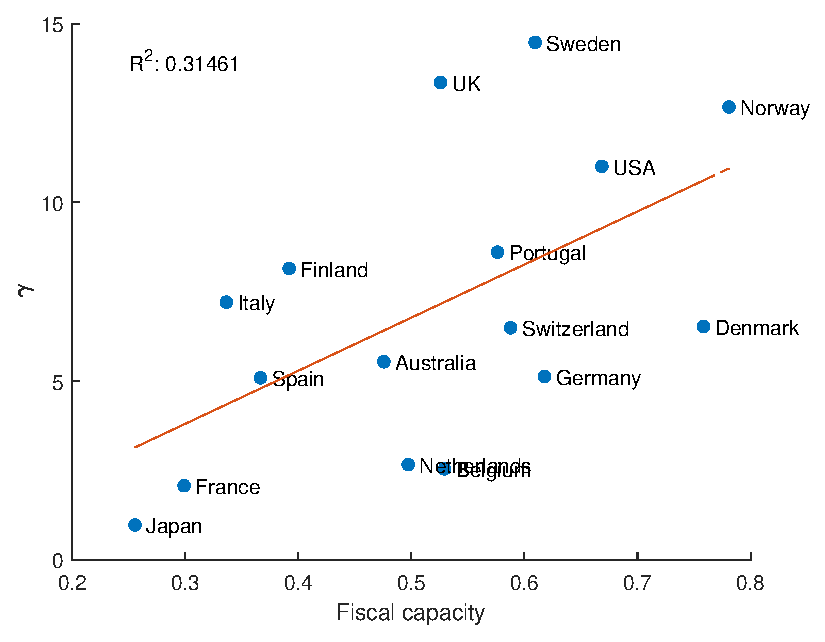
\includegraphics[width=0.7\textwidth]{Matlab Graphics/Fiscal_capacity}
	\caption{Standardized coefficients of variation, within-country tax revenue/GDP}
	\label{fig:fiscal_capacity}
\end{figure}
Figure \ref{fig:fiscal_capacity} above indicates that after controlling for disaster risk there is some variation stemming from fiscal capacity measured as the standardized coefficients of variation of within-country tax revenue/GDP. The higher the coefficient, the more the economic environment fluctuates and imposes distortions to financial markets, leading to liquidity premiums which leads to higher risk aversion. Further research could study different taxation types in the cross-section.

As \citet{Barro2006} suggests the analysis of real rates of return might include housing as component of the wealth portfolio as well. Given that such data is available \cite{Jorda2017} the implementation should be straight-forward.

\citet{Barro2006} and \citet{Nakamura2013} point at incorporating time-varying disaster moments which has been followed by \citet{Tsai2015}. The finding of \citet{Nakamura2013} on the role of the IES (especially at the onset of disasters) points at time-varying properties of the IES itself. Apart from dynamic aspects of disasters they also point out the distinction between actual and perceived disaster risks due to learning in order to alleviate the uncertainty regarding disaster parameters.
~\\
\newpage
\addcontentsline{toc}{section}{Acknowledgements}
\section*{Acknowledgements}
I want to thank my supervisor Wei Cui for valuable comments, guidance and steady support. I also want to thank Dr. Markus Baltzer and Dr. Philipp Lieberknecht for close cooperation and intellectual exchange. I want to thank Dr. Christian Speck for methodological advice and fruitful cooperation on data management as well as the entire directorate of general economics (division balance of payments, exchange rates and capital market analysis) at Deutsche Bundesbank for providing ideational and practical support.
\newpage
\bibliography{MasterThesisUCL.bib}
\addcontentsline{toc}{section}{References}

\bibliographystyle{apalike}
\setlength{\bibsep}{7pt}
\raggedright % beautify URLs
%\bibliography{MasterThesisUCL.bib}
\justify
\newpage
\addcontentsline{toc}{section}{Appendix}
\section*{Appendix}

{\renewcommand{\arraystretch}{1.5}
\begin{table}[H]
\begin{center}
\begin{tabular}{rccccc}
\hline
\hline
\multirow{2}{*}{Country} & \multirow{2}{*}{Equity} & \multirow{2}{*}{Bills} & GDP & Consumption & \multirow{2}{*}{Inflation}\\
& & & (per capita) & (per capita) &\\
\hline

Australia & 1870-2015 & 1870-2015 & 1870-2015 & 1870-2015 & 1870-2015 \\ 

Belgium & 1870-2015 & 1870-2015 & 1870-2015 & 1913-2015 & 1870-2015 \\ 

Denmark & 1873-2015 & 1875-2015 & 1870-2015 & 1870-2015 & 1870-2015 \\ 

Finland & 1896-2015 & 1870-2015 & 1870-2015 & 1870-2015 & 1870-2015 \\ 

France & 1870-2015 & 1870-2015 & 1870-2015 & 1870-2015 & 1870-2015 \\ 

Germany & 1870-2015 & 1870-2015 & 1870-2015 & 1870-2015 & 1870-2015 \\ 

Italy & 1870-2015 & 1885-2015 & 1870-2015 & 1870-2015 & 1870-2015 \\ 

Japan & 1886-2015 & 1876-2015 & 1870-2015 & 1870-2015 & 1870-2015 \\ 

Netherlands & 1900-2015 & 1870-2015 & 1870-2015 & 1870-2015 & 1870-2015 \\ 

Norway & 1881-2015 & 1870-2015 & 1870-2015 & 1870-2015 & 1870-2015 \\ 

Portugal & 1871-2015 & 1880-2015 & 1870-2015 & 1910-2015 & 1870-2015 \\ 

Spain & 1900-2015 & 1870-2015 & 1870-2015 & 1870-2015 & 1870-2015 \\ 

Sweden & 1871-2015 & 1870-2015 & 1870-2015 & 1870-2015 & 1870-2015 \\ 

Switzerland & 1900-2015 & 1900-2015 & 1870-2015 & 1870-2015 & 1870-2015 \\ 

United Kingdom & 1871-2015 & 1870-2015 & 1870-2015 & 1870-2015 & 1870-2015 \\ 

United States & 1872-2015 & 1870-2015 & 1870-2015 & 1870-2015 & 1870-2015 \\ 
\hline 
\hline
\end{tabular} 
\end{center}
\caption{Data coverage}
\label{tab:data_coverage}
\end{table}

{\renewcommand{\arraystretch}{1.0}
\begin{table}[H]
\begin{center}
\begin{tabular}{rccccccccccc}
\hline
\hline
Country & \multicolumn{5}{c}{Full sample (1870-2015)} & & \multicolumn{5}{c}{post-1984} \\
%\cline{2-6} \cline{8-12}
\hline
 & \multicolumn{2}{c}{Equity} & & \multicolumn{2}{c}{Bills} & & \multicolumn{2}{c}{Equity} & & \multicolumn{2}{c}{Bills}\\
\cline{2-3} \cline{5-6} \cline{8-9} \cline{11-12}
 & Mean & Std & & Mean & Std & & Mean & Std & & Mean & Std\\
\hline
Australia & 8.57 & 16.49 & & 1.98 & 4.47 & & 8.75 & 18.94 & & 3.62 & 2.48\\
Belgium & 5.99 & 22.92 & & 0.08 & 12.61 & & 11.92 & 24.90 & & 2.24 & 2.87 \\
Denmark & 7.89 & 17.41 & & 2.99 & 5.61 & & 10.84 & 21.53 & & 2.70 & 3.17 \\
Finland & 8.90 & 33.26 & & -1.45 & 14.90 & & 15.74 & 42.53 & & 2.84 & 3.65\\
France & 3.02 & 23.67 & & -1.32 & 9.58 & & 10.47 & 24.49 & & 2.45 & 2.71\\
Germany & 7.89 & 30.56 & & -2.57 & 27.64 & & 10.31 & 24.72 & & 1.86 & 1.92\\
Italy & 5.55 & 29.71& & -0.95 & 16.26 & & 9.99 & 29.99 & & 2.86 & 2.94\\
Japan & 6.83 & 35.76 & & -2.41 & 23.90 & & 5.46 & 22.63 & & 1.26 & 1.90\\
Netherlands & 7.26 & 22.65 & & 0.75 & 4.92 & & 10.69 & 22.81 & & 2.03 & 2.56 \\
Norway & 5.81 & 20.72 & & 0.81 & 6.04 & & 12.55 & 28.90 & & 2.19 & 1.86\\
Portugal & 3.87 & 28.93 & & -0.28 & 10.50 & & 11.41 & 39.75 & & 1.97 & 2.94 \\
Spain & 6.00 & 22.28 & & -0.37 &  7.15 & & 14.23 & 28.66 & & 2.39 & 3.54\\
Sweden & 8.17 & 20.45 & & 1.72 & 5.65 & & 13.55 & 28.24 & & 1.80 & 1.73\\
Switzerland & 6.50 & 19.41 & & 0.73 & 5.00 & & 10.12 & 22.53 & & 0.73 & 1.72 \\
United Kingdom & 7.11 & 19.37 & & 1.17 & 4.89 & & 8.67 & 15.64 & & 2.92 & 3.14\\
United States & 8.43 & 19.00 & & 2.15 & 4.62 & & 9.59 & 16.85 & & 1.67 & 2.36 \\
\hline
Average & 6.74 & - & & 0.20 & - & & 10.89 & - & & 2.22 & -\\
\hline
\hline
\end{tabular} 
\end{center}
\caption{Real rates of return (country-level), \%}
\label{tab:real_returns_countries}
\end{table}

{\renewcommand{\arraystretch}{1.0}
\begin{table}[H]
\begin{center}
\begin{tabular}{rccccc}
\hline
\hline
& \multicolumn{2}{c}{Equally weighted} & & \multicolumn{2}{c}{real GDP-weighted} \\
\cline{2-3} \cline{5-6}
& GDP & consumption & & GDP & consumption\\
\hline
Full sample & & & & &\\
\hline
Mean growth rate p.a. & 1.95 & 1.73 & & 1.93 & 1.70\\
Std.dev. & 1.17 & 1.39 & & 1.06 & 1.29\\
Geometric mean & 1.95 & 1.72 & & 1.93 & 1.70\\
Median & 1.97 & 1.84 & & 1.95 & 1.87\\
Max & 4.39 & 4.10 & & 4.09 & 4.02\\
Min & 0.21 & -1.26 & & 0.30 & -0.46\\
Kurtosis & 2.47 & 2.26 & & 2.13 & 1.89\\
\hline
Post-1984 & & & & &\\
\hline
Mean growth rate p.a. & 1.49 & 1.43 & & 1.51 & 1.59\\
Std.dev. & 0.78 & 0.69 & & 0.72 & 0.70\\
Geometric mean & 1.48 & 1.42 & & 1.51 & 1.59\\
Median & 1.96 & 1.79 & & 1.82 & 1.98\\
Max & 2.24 & 2.10 & & 2.43 & 2.42\\
Min & 0.21 & 0.24 & & 0.46 & 0.52\\
Kurtosis & 1.74 & 1.91 & & 1.50 & 1.61\\
\hline
\hline
\end{tabular} 
\end{center}
\caption{Global growth rates (1900-2015), \%, HP-filtered ($\lambda=100$)}
\label{tab:global_growth_HP}
\end{table}

{\renewcommand{\arraystretch}{1.0}
\begin{table}[H]
\begin{center}
\begin{tabular}{rccccccccccc}
\hline
\hline
Country & \multicolumn{5}{c}{Full sample (1870-2015)} & & \multicolumn{5}{c}{post-1984} \\
%\cline{2-6} \cline{8-12}
\hline
 & \multicolumn{2}{c}{GDP} & & \multicolumn{2}{c}{consumption} & & \multicolumn{2}{c}{GDP} & & \multicolumn{2}{c}{Consumption}\\
\cline{2-3} \cline{5-6} \cline{8-9} \cline{11-12}
 & Mean & Std & & Mean & Std & & Mean & Std & & Mean & Std\\
\hline
Australia & 1.45 & 1.30 & & 1.16 & 1.60 & & 1.83 & 0.51 & & 1.76 & 0.61\\
Belgium$^{*}$ & 1.66 & 2.10 & & 1.68 & 2.10 & & 1.41 & 0.68 & & 1.17 & 0.71 \\
Denmark & 1.69 & 1.06 & & 1.37 & 0.78 & & 1.06 & 0.64 & & 0.78 & 0.48 \\
Finland & 2.09 & 1.39 & & 2.12 & 1.39 & & 1.50 & 1.17 & & 1.80 & 0.77\\
France & 1.64 & 2.01 & & 1.42 & 2.10 & & 1.24 & 0.65 & & 1.23 & 0.52\\
Germany & 1.67 & 2.38 & & 1.67 & 2.31 & & 1.61 & 0.32 & & 1.30 & 0.64\\
Italy & 1.84 & 1.78 & & 1.49 & 1.97 & & 1.24 & 1.65 & & 0.82 & 1.49\\
Japan$^{*}$ & 2.46 & 2.64 & & 2.18 & 3.23 & & 1.42 & 1.05 & & 1.58 & 0.91\\
Netherlands & 1.57 & 1.72 & & 1.43 & 1.80 & & 1.60 & 0.84 & & 1.02 & 1.05 \\
Norway & 2.10 & 1.15 & & 1.84 & 0.81 & & 1.73 & 1.12 & & 2.16 & 0.64\\
Portugal$^{*}$ & 1.88 & 1.79 & & 2.36 & 1.94 & & 1.63 & 1.53 & & 2.17 & 1.91 \\
Spain & 1.81 & 1.98 & & 1.51 &  2.18 & & 1.84 & 1.58 & & 1.32 & 1.57\\
Sweden & 2.02 & 0.91 & & 1.80 & 0.72 & & 1.51 & 0.58 & & 1.14 & 0.42\\
Switzerland & 1.38 & 1.07 & & 1.27 & 0.90 & & 0.94 & 0.27 & & 0.80 & 0.17\\
United Kingdom & 1.39 & 0.81 & & 1.32 & 0.97 & & 1.66 & 0.82 & & 1.95 & 1.12\\
United States & 1.94 & 1.33 & & 1.77 & 1.04 & & 1.53 & 0.65 & & 1.81 & 0.64 \\
\hline
Average & 1.79 & - & &  & - & & 1.49 & - & &  & -\\

\hline
\hline
\multicolumn{12}{c}{$^{*}$ Belgium: 1914-2015, Japan: 1875-2015, Portugal: 1911-2015}
\end{tabular} 
\end{center}
\caption{Real growth rates (country-level), \%, HP-filtered ($\lambda=100$)}
\label{tab:real_growth_countries_HP}
\end{table}

%\begin{python}
%\caption{Peak-to-trough code}
%\label{code}
%\end{python}

\begin{python}
data = pd.read_excel(<ENTER DATASET HERE>, sheet_name = 'C JST')
data['year'] = data['C pc']
del data['C pc']
data = data.iloc[1:]
data.set_index('year', inplace=True, drop=True)
start_year = 1870
end_year = 2015
data = data.loc[start_year:end_year];
threshold = 0.095
countries = list(data.columns)
years = list(data.index)
data_pct = data.pct_change()
cons_df = data_pct
country_list = []
disaster_df_list = []
for country in countries:
    country_dict = {}
    sub_frame = data_pct[country]
    total_years = len(sub_frame.dropna())
    sub_frame_less = sub_frame.iloc[1:]
    na_index = sub_frame_less.loc[pd.isna(sub_frame_less)].index
    succession_counter = 0
    succession_container = []
    succession_year_container = []
    
    for x in years:
        if x+1 <= end_year and sub_frame.loc[x] < 0 and sub_frame.loc[x+1] < 0:
        
        	succession_counter += 1
            if succession_counter == 1:
                
                empty_list = [sub_frame.loc[x], sub_frame.loc[x+1]]
                empty_year_list = [x, x+1]
                
            elif succession_counter > 1:
                
                empty_list.append(sub_frame.loc[x+1])
                empty_year_list.append(x+1)
                
            succession_container.append(empty_list)
            succession_year_container.append(empty_year_list)
                   
        else:
      
            succession_counter = 0
        
    unique_periods = list(succession_year_container for succession_year_container,_ in itertools.groupby(succession_year_container))
    
    cumulative_contractions = []
    
    for i in list(succession_container for succession_container,_ in itertools.groupby(succession_container)):
        
        cumulative_contractions.append(sum(i))
        
    empty_check_list = []

    for idx, i in enumerate(cumulative_contractions):
    
        empty_dict = {}
    
        if i <= - threshold:
        
            empty_dict['contraction'] = i
            empty_dict['index'] = idx
			empty_check_list.append(empty_dict)
            
    disaster_df = pd.DataFrame(empty_check_list)
            
    disaster_periods = []

    for i in list(disaster_df['index'].values):
    
        disaster_periods.append(unique_periods[i])
        
    disaster_df['period'] = disaster_periods
    disaster_df['country'] = country
        
    flat_list = []
    for sublist in disaster_periods:
        for item in sublist:
            flat_list.append(item)          
            
    single_years = sub_frame[sub_frame <= - threshold]
    single_year_list = []

    for idx, i in enumerate(single_years.index):
    
        if i not in flat_list:
        
            single_year_list.append(i)
    
    left_over_df = pd.DataFrame(single_years[single_year_list])
    left_over_df.reset_index(drop = False, inplace = True)
    left_over_df.columns = ['period', 'contraction']
    left_over_df['country'] = country
    del disaster_df['index']
    final_df = disaster_df.append(left_over_df)
    final_df.reset_index(inplace=True, drop = True)
    disaster_df_list.append(final_df)
    total_number_disasters = len(final_df)
    flattened_years = []

    for i in range(len(final_df)):
    
        sub_years = final_df['period'][i]
    
        if type(sub_years) != int:
        
            sub_years = [str(item) for item in sub_years]
        
            for x in sub_years:
            
                flattened_years.append(x)
        
        elif type(sub_years) == int:
        
            flattened_years.append(str(sub_years))
            
    total_number_disaster_years = len(flattened_years)
    average_disaster_size = abs(final_df['contraction'].mean())
    non_disaster_years = total_years-total_number_disaster_years
    disaster_probability = total_number_disasters / non_disaster_years
    
    country_dict['Country'] = country
    country_dict['no disasters'] = total_number_disasters
    country_dict['no disaster years'] = total_number_disaster_years
    country_dict['average disaster size'] = average_disaster_size
    country_dict['no non-disaster years'] = non_disaster_years
    country_dict['disaster probability'] = disaster_probability
    country_dict['annual average growth rate'] = sub_frame.mean()
    country_dict['standard deviation annual growth rate'] = sub_frame.std()
    country_dict['kurtosis'] = sub_frame.kurtosis()
    country_dict['total years'] = total_years
    country_dict['missing years'] = np.NaN
    country_dict['number missing years'] = np.NaN
    
    if len(na_index) != 0:
        
        missing_years = sub_frame_less.loc[na_index]
        country_dict['missing years'] = list(sub_frame_less.loc[na_index].index)
        country_dict['number missing years'] = len(missing_years)
  
    country_list.append(country_dict)
    
consumption_disaster_df = pd.DataFrame(country_list)
consumption_disaster_events = pd.concat(disaster_df_list)
\end{python}
\begin{lstlisting}[frame=none,caption={Peak-to-trough algorithm},captionpos=b,label=lst:code]
\end{lstlisting}



{\renewcommand{\arraystretch}{1.0}
\begin{table}[H]
\begin{center}
\begin{tabular}{rccccc}
\hline
\hline
\multirow{3}{*}{Country} & \multirow{3}{*}{\shortstack{No.\\disasters}} & \multirow{3}{*}{\shortstack{No.\\disaster\\years}} & \multirow{3}{*}{\shortstack{No. non-\\disaster\\years}} & \multirow{3}{*}{\shortstack{Disaster\\probability\\(\%)}} & \multirow{3}{*}{\shortstack{Average\\disaster size\\(\%)}}\\
& & & & &\\
& & & & &\\
\hline
Australia & 4 & 15 & 130 & 3.08 & 18.18\\
Belgium$^{*}$ & 5 & 13 & 132 & 3.79 & 27.59\\
Denmark & 2 & 4 & 141 & 1.42 & 18.50\\
Finland & 5 & 15 & 130 & 3.85 & 15.48\\
France & 7 & 21 & 124 & 5.65 & 19.11\\
Germany & 4 & 14 & 131 & 3.05 & 44.03\\
Italy & 2 & 8 & 137 & 1.46 & 36.17\\
Japan$^{*}$ & 2 & 8 & 137 & 1.46 & 35.19\\
Netherlands & 3 & 15 & 130 & 2.31 & 35.92\\
Norway & 3 & 6 & 139 & 2.16 & 13.23\\
Portugal$^{*}$ & 2 & 3 & 142 & 1.41 & 13.14\\
Spain & 4 & 13 & 132 & 3.03 & 16.73\\
Sweden & 3 & 5 & 140 & 2.14 & 11.90\\
Switzerland & 3 & 9 & 136 & 2.21 & 16.09\\
United Kingdom & 2 & 7 & 138 & 1.45 & 18.05\\
United States & 5 & 13 & 132 & 3.79 & 16.45\\
\hline
$\Sigma$ & 56 & 169 & 2,151 & 2.60 & $\mu=22.23$\\
\hline
\hline
\multicolumn{6}{c}{$^{*}$ Belgium: 1914-2015, Japan: 1875-2015, Portugal: 1911-2015}
\end{tabular} 
\end{center}
\caption{Disaster risk moments (GDP)}
\label{tab:disaster_risk_gdp}
\end{table}

\begin{figure}[H]
	\centering
  \includegraphics[width=\textwidth]{Graphics/Gantt_GDP_highres.PNG}
	\caption{GDP disasters across countries over time}
	\label{fig:Gant_GDP}
\end{figure}

{\renewcommand{\arraystretch}{1.0}
\begin{table}[H]
\begin{center}
\begin{tabular}{rccccc}
\hline
\hline
Country & \multicolumn{2}{c}{Consumption} & & \multicolumn{2}{c}{GDP} \\
%\cline{2-6} \cline{8-12}
\cline{2-3} \cline{5-6} 
 & $g$ & $\sigma$ & & $g$ & $\sigma$\\
\hline
Australia & 2.51 & 4.41 &  & 2.28 & 3.44\\
Belgium & 3.46 & 6.34 &  & 3.17 & 7.03\\
Denmark & 2.08 & 4.36 &  & 2.07 & 3.13\\ 
Finland & 3.36 & 4.31 &  & 3.02 & 3.69\\ 
France & 2.41 & 5.30 &  & 3.24 & 4.94\\ 
Germany & 3.08 & 4.22 &  & 3.66 & 4.20\\
Italy & 1.83 & 3.35 &  & 2.56 & 3.58\\
Japan & 3.18 & 5.41 &  & 3.28 & 4.77\\
Netherlands & 2.82 & 6.89 &  & 2.83 & 6.57\\
Norway & 2.37 & 3.11 &  & 2.56 & 3.06\\ 
Portugal & 3.20 & 3.82 &  & 2.17 & 3.98\\
Spain & 4.24 & 5.52 &  & 2.70 & 4.11\\
Sweden & 2.17 & 4.04 &  & 2.43 & 2.81\\
Switzerland & 2.36 & 5.22 &  & 1.95 & 3.45\\
United Kingdom & 1.71 & 2.32 &  & 1.78 & 2.43\\
United States & 2.23 & 3.11 &  & 2.87 & 4.12\\
\hline
\hline
\end{tabular} 
\end{center}
\caption{Growth rates (non-disaster years), \%}
\label{tab:growth_non_disaster}
\end{table}

{\renewcommand{\arraystretch}{1.0}
\begin{table}[H]
\begin{center}
\begin{tabular}{rccccccc}
\hline
\hline
Country & $g^{*}$ (\%) & $\rho^{*}$ & $\beta^{*}$ & $r^{e}$ (\%) & $r^{f}$ (\%) & \underline{$\gamma$} & \boldsymbol{$\gamma$}\\
\hline

Australia & 1.78 & 0.0414 & 0.9603 & 6.98 & 2.58 & 39.18 & 9.58\\ 

Belgium & 2.37 & 0.0328 & 0.9683 & 7.30 & 3.36 & 8.88 &  3.51\\ 

Denmark & 1.86 & -0.0142 & 1.0144 & 6.80 & 3.54 & 36.61 &  10.94\\ 

Finland & 2.50 & 0.0529 & 0.9498 & 7.76 & 0.86 & 50.99 &  13.42\\ 

France & 2.28 & 0.0115 & 0.9887 & 7.04 & 4.15 & 11.10 &  4.59\\ 

Germany & 2.40 & 0.0501 & 0.9523 & 7.61 & 0.64 & 16.70 &  3.03\\ 

Italy & 2.10 & 0.0248 & 0.9758 & 7.03 & 2.70 & 29.69 &  4.65\\ 

Japan & 2.88 & 0.0106 & 0.9895 & 7.72 & 1.56 & 25.89 &  5.44\\ 

Netherlands & 2.21 & 0.0385 & 0.9629 & 7.23 & 2.89 & 11.94 &  3.37\\ 

Norway & 2.32 & -0.0872 & 1.0956 & 7.09 & 3.75 & 39.36 &  14.57\\ 

Portugal & 2.07 & -0.0413 & 1.0431 & 6.93 & 4.16 & 22.95 &  12.12\\ 

Spain & 2.28 & -0.0003 & 1.0003 & 7.26 & 3.02 & 26.49 &  9.87\\ 

Sweden & 2.21 & -0.0628 & 1.0670 & 7.17 & 2.87 & 56.16 &  19.50\\ 

Switzerland & 1.66 & 0.0345 & 0.9667 & 6.84 & 3.00 & 38.42 &  11.77\\ 

United Kingdom & 1.55 & 0.0231 & 0.9774 & 6.69 & 2.73 & 72.30 &  12.96\\ 

United States & 2.33 & -0.0015 & 1.0015 & 7.28 & 3.10 & 26.47 &  9.19\\
\hline
Global & & & & & & &\\
\hline 
\hline
\end{tabular} 
\end{center}
\caption{Calibration \& results (GDP)}
\label{tab:results_GDP}
\end{table}

\begin{figure}[H]
	\begin{tabular}{cc}
	\subfloat[Expected rates of return on equity]{
		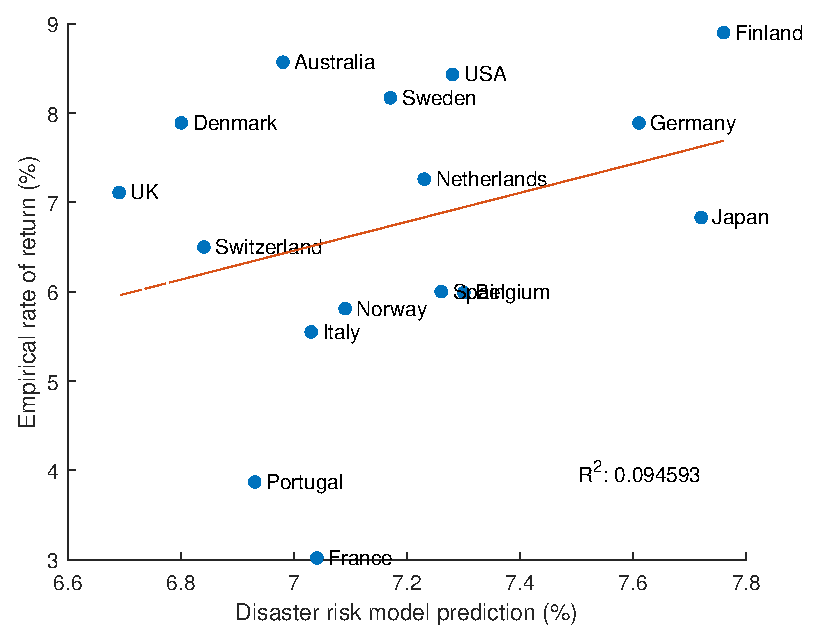
\includegraphics[width = 0.45\textwidth]{Matlab Graphics/Actual_vs_predicted_equity_GDP}
	} &
	\subfloat[Risk-free rates]{
		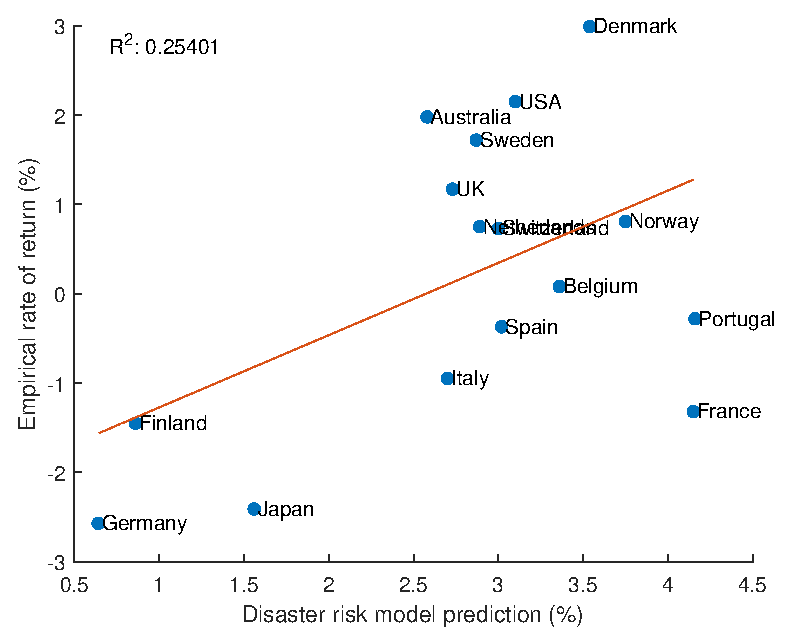
\includegraphics[width = 0.45\textwidth]{Matlab Graphics/Actual_vs_predicted_riskfree_GDP}
	}\\
	\end{tabular}
	\caption{Actual vs. predicted rates of return (GDP data)}
	\label{fig:actual_vs_predicted_rates_GDP}
\end{figure}

{\renewcommand{\arraystretch}{1.0}
\begin{table}[H]
\begin{center}
\begin{tabular}{rccccc}
\hline
\hline
\multirow{3}{*}{Country} & \multirow{3}{*}{\shortstack{No.\\disasters}} & \multirow{3}{*}{\shortstack{No.\\disaster\\years}} & \multirow{3}{*}{\shortstack{No. non-\\disaster\\years}} & \multirow{3}{*}{\shortstack{Disaster\\probability\\(\%)}} & \multirow{3}{*}{\shortstack{Average\\disaster size\\(\%)}}\\
& & & & &\\
& & & & &\\
\hline
\multicolumn{6}{c}{Consumption}\\
\hline
Australia & 6 & 17 & 128 & 4.69 & 22.60\\
Belgium$^{*}$ & 3 & 8 & 94 & 3.19 & 42.82\\
Denmark & 2 & 4 & 141 & 1.42 & 26.20\\
Finland & 3 & 10 & 135 & 2.22 & 27.85\\
France & 2 & 8 & 137 & 1.46 & 49.83\\
Germany & 2 & 12 & 133 & 1.50 & 50.82\\
Italy & 1 & 5 & 140 & 0.71 & 32.13\\
Japan$^{*}$ & 1 & 8 & 133 & 0.75 & 90.35\\
Netherlands & 3 & 10 & 135 & 2.22 & 42.14\\
Norway & 2 & 4 & 141 & 1.42 & 16.88\\
Portugal$^{*}$ & 1 & 5 & 100 & 1.00 & 23.47\\
Spain & 5 & 16 & 129 & 3.88 & 24.18\\
Sweden & 1 & 3 & 142 & 0.70 & 16.43\\
Switzerland & 4 & 11 & 134 & 2.99 & 19.52\\
United Kingdom & 2 & 8 & 137 & 1.46 & 17.72\\
United States & 2 & 8 & 137 & 1.46 & 20.02\\
\hline
$\Sigma$ & 40 & 137 & 2,096 & 1.90 & $\mu=32.69$\\
\hline
 & & & & & \\
  & & & & & \\
\hline
\multicolumn{6}{c}{GDP}\\
\hline
Australia & 3 & 10 & 135 & 2.22 & 20.45\\
Belgium$^{*}$ & 4 & 9 & 136 & 2.94 & 31.44\\
Denmark & 1 & 2 & 143 & 0.70 & 25.43\\
Finland & 1 & 2 & 143 & 0.70 & 29.94\\
France & 5 & 12 & 133 & 3.76 & 21.86\\
Germany & 3 & 13 & 132 & 2.27 & 54.14\\
Italy & 2 & 8 & 137 & 1.46 & 36.17\\
Japan$^{*}$ & 1 & 6 & 139 & 0.72 & 60.88\\
Netherlands & 2 & 10 & 135 & 1.48 & 47.09\\
Norway & 1 & 2 & 143 & 0.70 & 15.31\\
Portugal$^{*}$ & 1 & 2 & 143 & 0.70 & 15.40\\
Spain & 1 & 3 & 142 & 0.70 & 32.86\\
Sweden & 1 & 2 & 143 & 0.70 & 15.39\\
Switzerland & 2 & 6 & 139 & 1.44 & 17.55\\
United Kingdom & 2 & 7 & 138 & 1.45 & 18.05\\
United States & 2 & 7 & 138 & 1.45 & 24.80\\
\hline
$\Sigma$ & 32 & 101 & 2,219 & 1.44 & $\mu=29.17$\\
\hline
\hline
\multicolumn{6}{c}{$^{*}$ Belgium: 1914-2015, Japan: 1875-2015, Portugal: 1911-2015}
\end{tabular} 
\end{center}
\caption{Disaster risk moments (disaster threshold = 0.15)}
\label{tab:disaster_risk_threshold}
\end{table}


{\renewcommand{\arraystretch}{1.0}
\begin{table}[H]
\begin{center}
\begin{tabular}{rccccc}
\hline
\hline
\multirow{3}{*}{Country} & \multirow{3}{*}{\shortstack{No.\\disasters}} & \multirow{3}{*}{\shortstack{No.\\disaster\\years}} & \multirow{3}{*}{\shortstack{No. non-\\disaster\\years}} & \multirow{3}{*}{\shortstack{Disaster\\probability\\(\%)}} & \multirow{3}{*}{\shortstack{Average\\disaster size\\(\%)}}\\
& & & & &\\
& & & & &\\
\hline
\multicolumn{6}{c}{Consumption}\\
\hline
Australia & 2 & 26 & 119 & 1.68 & 19.01\\
Belgium$^{*}$ & 1 & 12 & 90 & 1.11 & 32.44\\
Denmark & - & - & - & - & -\\
Finland & - & - & - & - & -\\
France & 1 & 13 & 132 & 0.76 & 34.17\\
Germany & 2 & 20 & 125 & 1.60 & 21.67\\
Italy & 2 & 25 & 120 & 1.67 & 11.20\\
Japan$^{*}$ & 1 & 18 & 123 & 0.81 & 53.38\\
Netherlands & 1 & 10 & 135 & 0.74 & 20.88\\
Norway & - & - & - & - & -\\
Portugal$^{*}$ & 1 & 8 & 97 & 1.03 & 9.57\\
Spain & 1 & 12 & 133 & 0.75 & 26.90\\
Sweden & - & - & - & - & -\\
Switzerland & - & - & - & - & -\\
United Kingdom & - & - & - & - & -\\
United States & - & - & - & - & -\\
\hline
$\Sigma$ & 12 & 144 & 1,074 & 1.12 & $\mu=25.47$\\
\hline
 & & & & & \\
  & & & & & \\
\hline
\multicolumn{6}{c}{GDP}\\
\hline
Australia & 1 & 12 & 133 & 0.75 & 15.97\\
Belgium$^{*}$ & 2 & 21 & 124 & 1.61 & 19.51\\
Denmark & - & - & - & - & -\\
Finland & - & - & - & - & -\\
France & 1 & 12 & 133 & 0.75 & 23.79\\
Germany & 2 & 20 & 125 & 1.60 & 25.85\\
Italy & - & - & - & - & -\\
Japan$^{*}$ & 1 & 8 & 137 & 0.73 & 21.08\\
Netherlands & 1 & 13 & 132 & 0.76 & 20.92\\
Norway & - & - & - & - & -\\
Portugal$^{*}$ & - & - & - & - & -\\
Spain & 1 & 10 & 135 & 0.74 & 18.12\\
Sweden & - & - & - & - & -\\
Switzerland & - & - & - & - & -\\
United Kingdom & - & - & - & - & -\\
United States & - & - & - & - & -\\
\hline
$\Sigma$ & 9 & 96 & 919 & 0.98 & $\mu=20.75$\\
\hline
\hline
\multicolumn{6}{c}{$^{*}$ Belgium: 1914-2015, Japan: 1875-2015, Portugal: 1911-2015}
\end{tabular} 
\end{center}
\caption{Disaster risk moments (HP-filtered trend, $\lambda=100$)}
\label{tab:disaster_risk_HP}
\end{table}


{\renewcommand{\arraystretch}{1.0}
\begin{table}[H]
\begin{center}
\begin{tabular}{rccccccc}
\hline
\hline
Country & $g^{*}$ (\%) & $\rho^{*}$ & $\beta^{*}$ & $r^{e}$ (\%) & $r^{f}$ (\%) & \underline{$\gamma$} & \boldsymbol{$\gamma$}\\
\hline
\multicolumn{8}{c}{Consumption}\\
\hline

Australia & 1.73 & 0.0033 & 0.9967 & 3.33 & -1.07 & 20.10 & 12.63\\ 

Belgium & 1.91 & 0.0087 & 0.9914 & 6.79 & 2.85 & 7.91 &  6.25\\ 

Denmark & - & - & - & - & - & - &  -\\ 

Finland & - & - & - & - & - & - &  -\\  

France & 1.57 & 0.0143 & 0.9859 & 6.48 & 3.58 & 10.17 &  5.85\\ 

Germany & 1.96 & 0.0621 & 0.9416 & 6.24 & 6.24 & 34.08 &  0.02\\ 

Italy & 1.82 & -0.0593 & 1.0630 & 6.85 & 2.52 & 47.37 &  25.18\\ 

Japan & 2.54 & 0.0234 & 0.9771 & 7.32 & 1.16 & 20.62 &  3.52\\ 

Netherlands & 1.54 & 0.0603 & 0.9431 & 6.04 & 6.03 & 9.41 &  0.00\\ 

Norway & - & - & - & - & - & - &  -\\  

Portugal & 2.57 & -0.4229 & 1.7327 & 7.02 & 4.26 & 21.17 &  29.87\\ 

Spain & 1.67 & 0.0083 & 0.9917 & 6.69 & 2.44 & 11.23 &  9.60\\ 

Sweden & - & - & - & - & - & - &  -\\  

Switzerland & - & - & - & - & - & - &  -\\   

United Kingdom & - & - & - & - & - & - &  -\\  

United States & - & - & - & - & - & - &  -\\  
\hline
Global & & & & & & &\\
\hline
 & & & & & \\
  & & & & & \\
\hline
\multicolumn{8}{c}{GDP}\\
\hline
Australia & 1.59 & 0.0606 & 0.9429 & 6.06 & 6.06 & 39.18 & 0.00\\ 

Belgium & 1.95 & -0.0296 & 1.0305 & 6.85 & 2.90 & 8.88 &  11.66\\ 

Denmark & - & - & - & - & - & - &  -\\ 

Finland & - & - & - & - & - & - &  -\\ 

France & 1.80 & -0.0367 & 1.0381 & 6.60 & 3.70 & 11.10 &  10.07\\ 

Germany & 1.95 & 0.0619 & 0.9417 & 6.24 & 6.23 & 16.70 &  0.02\\ 

Italy & - & - & - & - & - & - &  -\\ 

Japan & 2.63 & 0.0655 & 0.9386 & 6.58 & 6.58 & 25.89 &  0.01\\ 

Netherlands & 1.74 & 0.0613 & 0.9423 & 6.13 & 6.13 & 11.94 &  0.00\\ 

Norway & - & - & - & - & - & - &  -\\  

Portugal & - & - & - & - & - & - &  -\\ 

Spain & 1.96 & 0.0618 & 0.9418 & 6.25 & 6.24 & 26.49 &  0.03\\ 

Sweden & - & - & - & - & - & - &  -\\ 

Switzerland & - & - & - & - & - & - &  -\\ 

United Kingdom & - & - & - & - & - & - &  -\\  

United States & - & - & - & - & - & - &  -\\ 
\hline
Global & & & & & & &\\
\hline 
\hline
\end{tabular} 
\end{center}
\caption{Calibration \& results (HP-filtered trend, $\lambda=100$)}
\label{tab:results_HP}
\end{table}











\newpage
\section*{Statutory Declaration}
I hereby declare that except where specific reference is made to the work of 
others, the contents of this thesis are original and have not been 
submitted in whole or in part for consideration for any other degree or 
qualification in this, or any other university. This thesis is my own 
work and contains nothing which is the outcome of work done in collaboration 
with others, except as specified in the text and Acknowledgements. This 
dissertation contains fewer than 10,000 words excluding bibliography and appendices.

\flushright
Gerome Wolf\\
\today
\vfill
\end{document}